\documentclass{article}
\usepackage[utf8]{inputenc}
\usepackage{graphicx}
\usepackage{amsmath}
\graphicspath{ {./Images/} }
\usepackage{float}

\title{CTA200 Computing Project}
\author{Caleb Lammers}
\date{May 19 2020}

\begin{document}

\maketitle

\section*{Introduction}

The light emitted from a galaxy provides information about its physical properties, including both
its star formation history and stellar mass. Light emitted from galaxies' in different wavelengths
contain different information about the galaxy's composition. For instance, it is well known that
younger stars emit shorter wavelength light, that is, bluer light than old stars. Thus, if a galaxy
emits much more shorter wavelength light, this galaxy likely has many younger stars and thus was forming
stars not so long ago. Because different wavelengths help provide different insights, it is useful
to represent a galaxy's emitted light as a graph of luminosity/flux density vs. wavelength, called
the galaxy's Spectral Energy Distribution (SED).

\begin{figure}[h]
  \centering
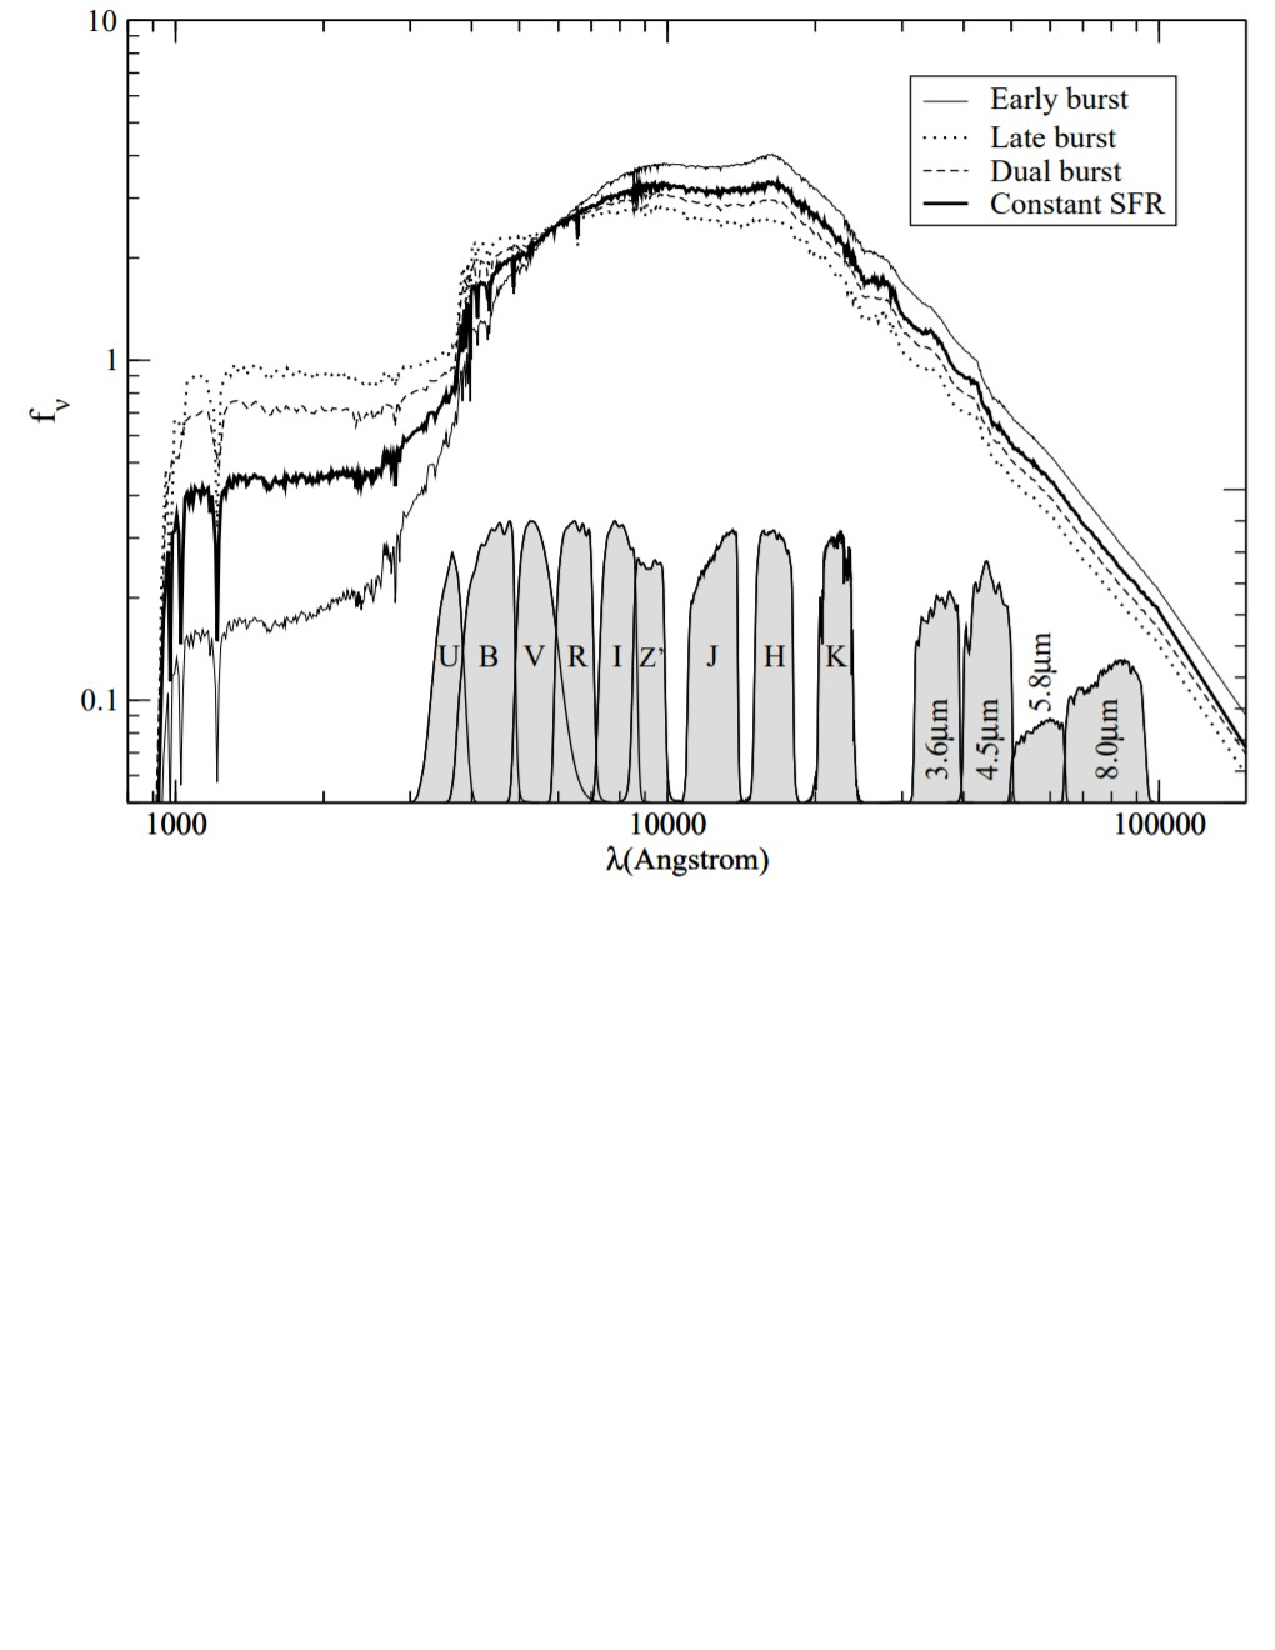
\includegraphics[scale=0.4]{SED Example}
\caption{Example SED of flux density vs. wavelength}
\end{figure}

By combining knowledge on stellar evolution, calibrated stellar libraries, initial mass functions
(IMF), and dust in the interstellar medium, it is possible to predict the SED of galaxies, based on
their physical properties. This is known as stellar population synthesis (SPS) and mode that
combines these ingredients is called a stellar population synthesis model. In this project,
the FSPS (Conroy and Gunn 2009) SPS model was used, particularly the python package python-FSPS.
Being able to compute a galaxies' SED based on its physical properties is a step in the right direction,
however, as astronomers, we would like to be able to determine a galaxy's physical properties from
its observable SED. This project will consist of two parts. In the first, the FSPS model was set up
and functions were created so that SEDs and other important graphs could be made. In the second,
the goal was to work backwards and determine the physical properties of two galaxies, given their SEDs, which was done using
brute force and Markov chain Monte Carlo (MCMC) methods.

\section*{Description of Script}
\subsection*{Part 1}

A StellarPopulation object was initialized in accordance with the settings provided in question 4.
Now, by using the built in get spectrum method, SEDs of (bolometric) luminosity in $L_\odot/Hz$
vs. wavelength in $\AA$ can be made.

\begin{figure}[h]
  \centering
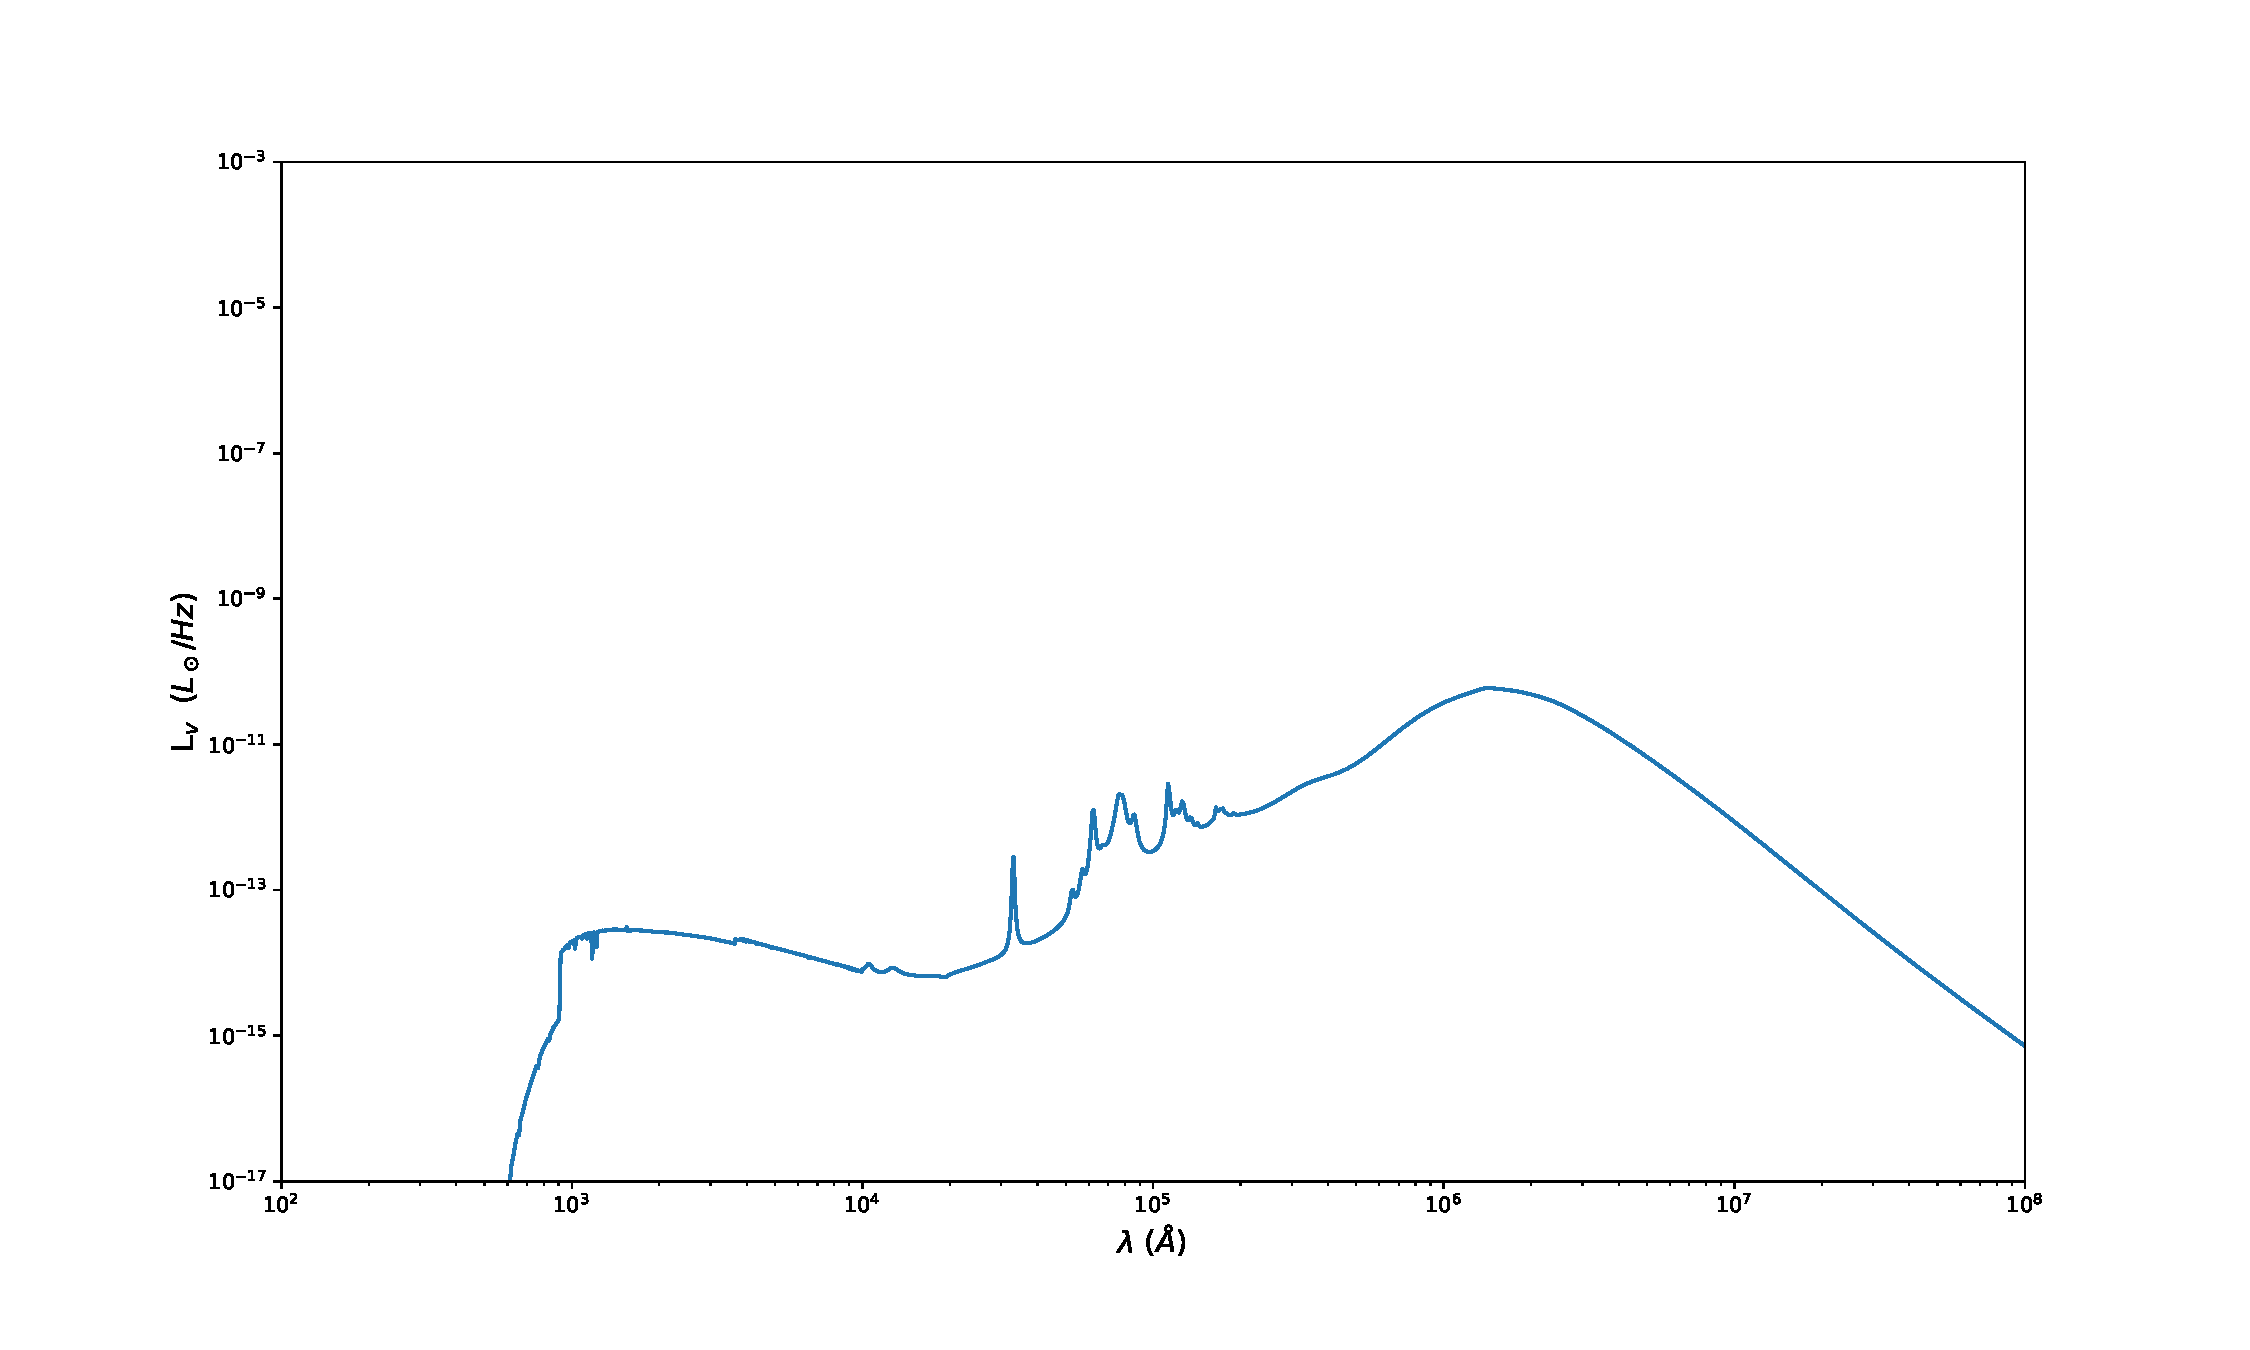
\includegraphics[scale=0.3]{SED Default Units}
\caption{SED of luminosity vs. wavelength}
\end{figure}


SEDs are more commonly presented as flux density (in $\mu Jy$) vs wavelength (in $\AA$), so, next a
function was written to convert the SED from units of luminosity into units of spectral flux,
according to the equation below.

\begin{figure}[H]
\[\textrm{f}_v = \frac{\textrm{L}_{(1 + z)v}}{4\pi D_L^2} \]
\caption{Flux density from luminosity}
\end{figure}

Because $\textrm{f}_v$ depends on $(1 + z)v$ rather than $v$, instead of converting each $\textrm{f}_v$
into $\textrm{L}_v$, it is easier to convert $\textrm{f}_v$ to $\textrm{L}_{(1 + z)v}$
and scale each $\lambda$ by $(1 + z)$. Now, SEDs of this galaxy can be created in units of spectral flux by specifying a redshift. Note
that at all redshifts we expect the SED to have similar behaviour as above because we have only
rescaled the x and y axes.

\begin{figure}[H]
  \centering
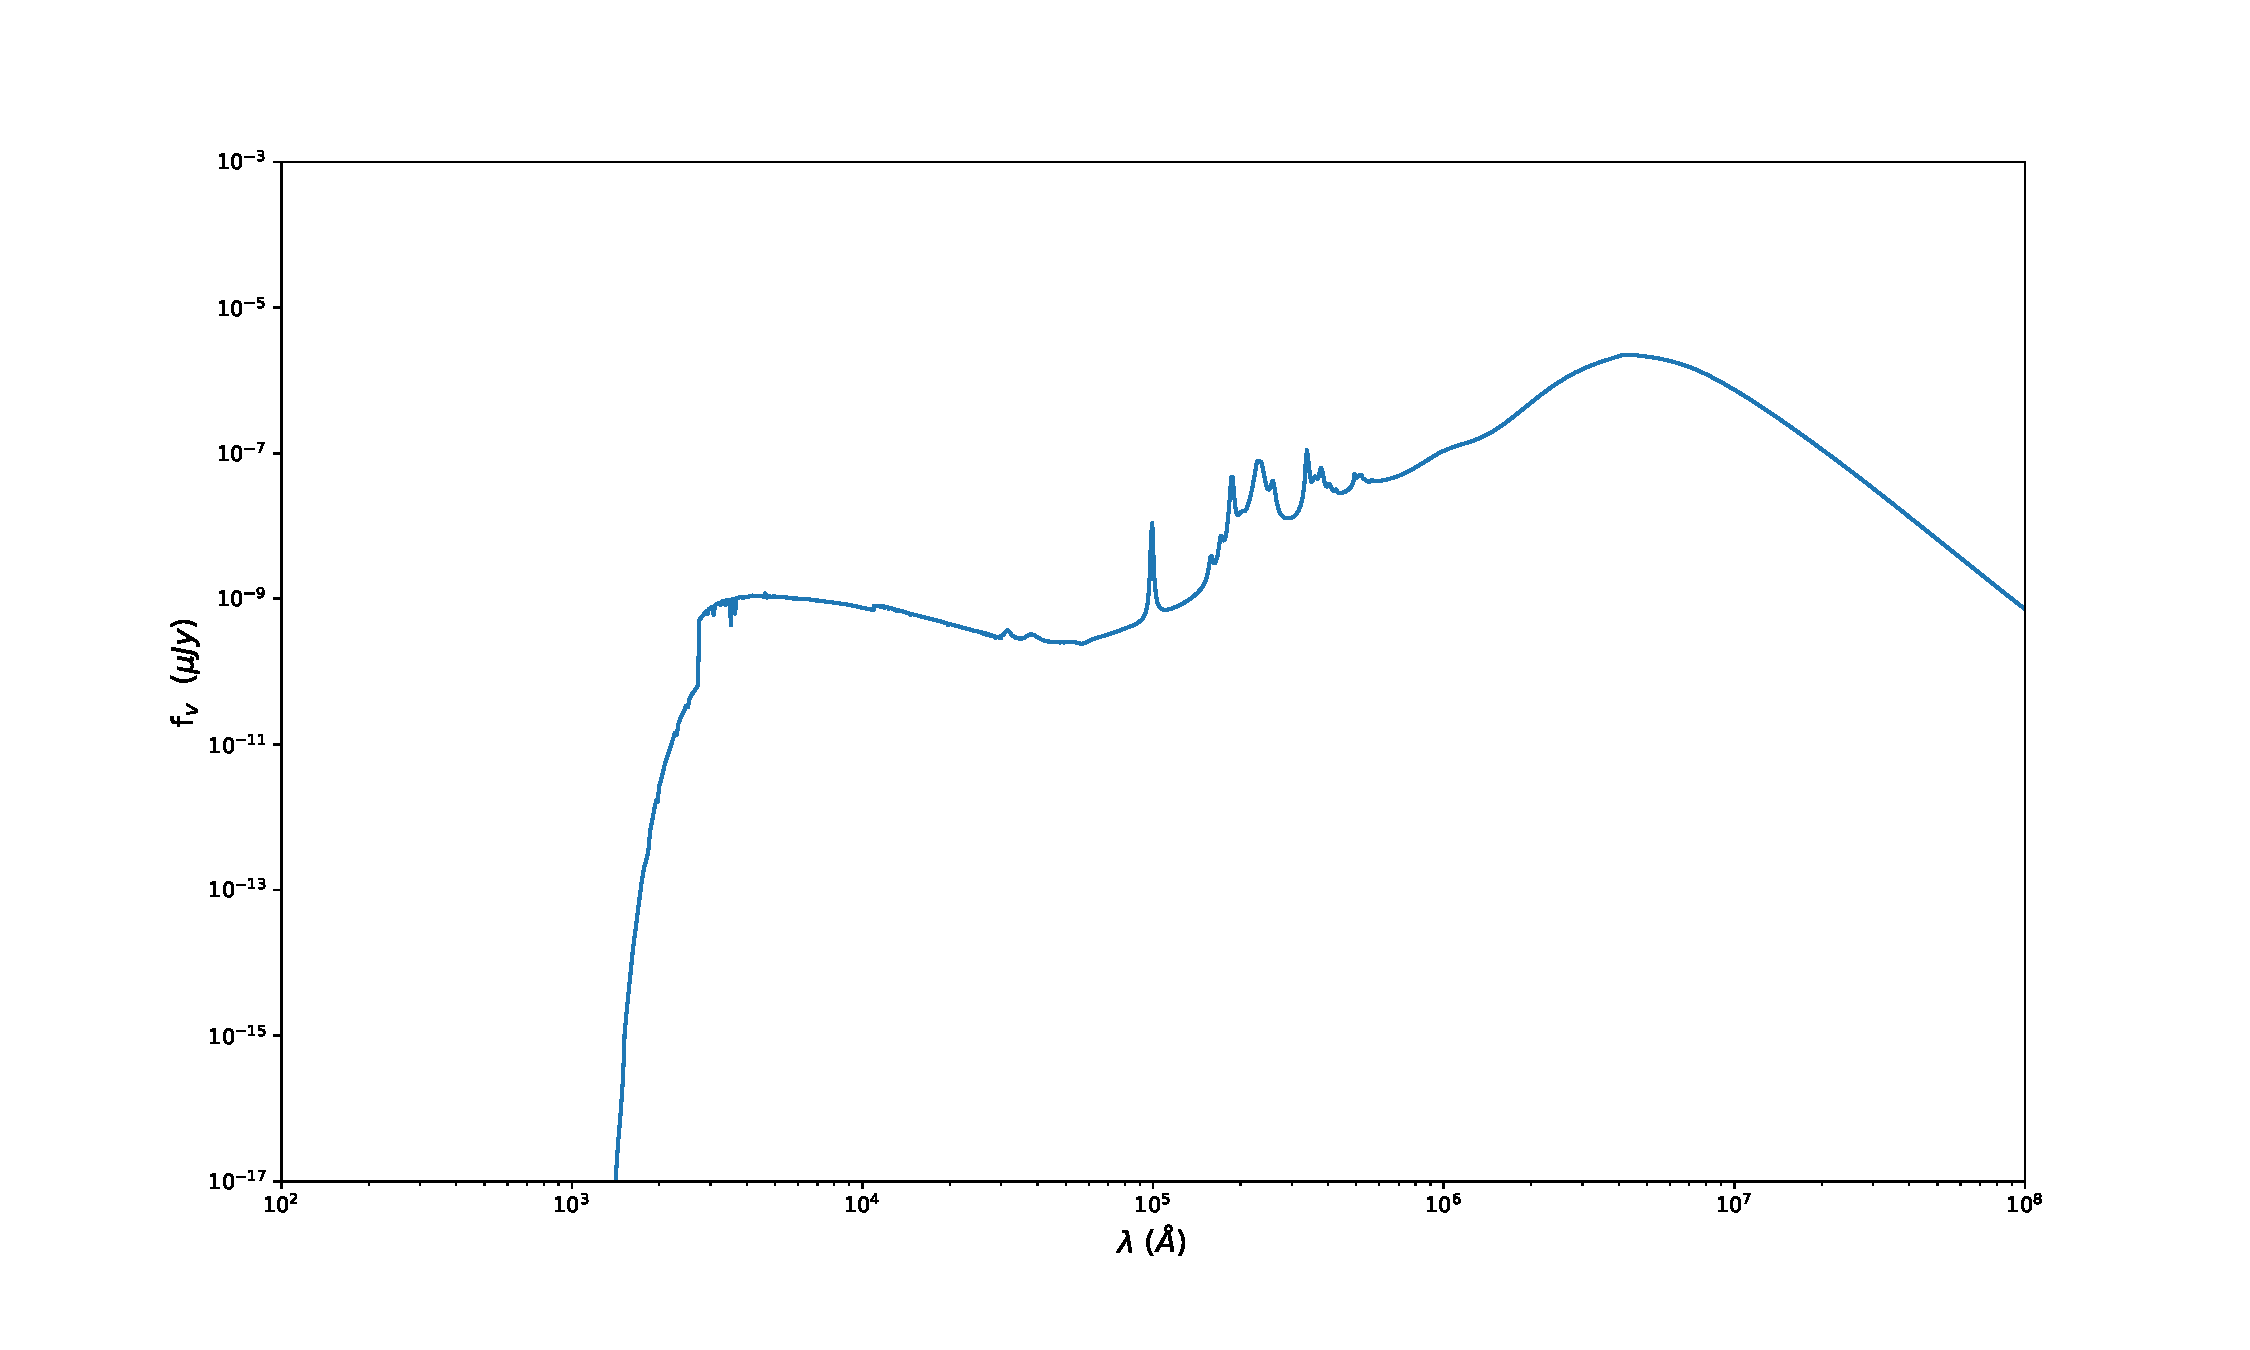
\includegraphics[scale=0.3]{SED redshift 1}
\caption{SED of flux density vs. wavelength at redshift 1}
\end{figure}

\begin{figure}[H]
  \centering
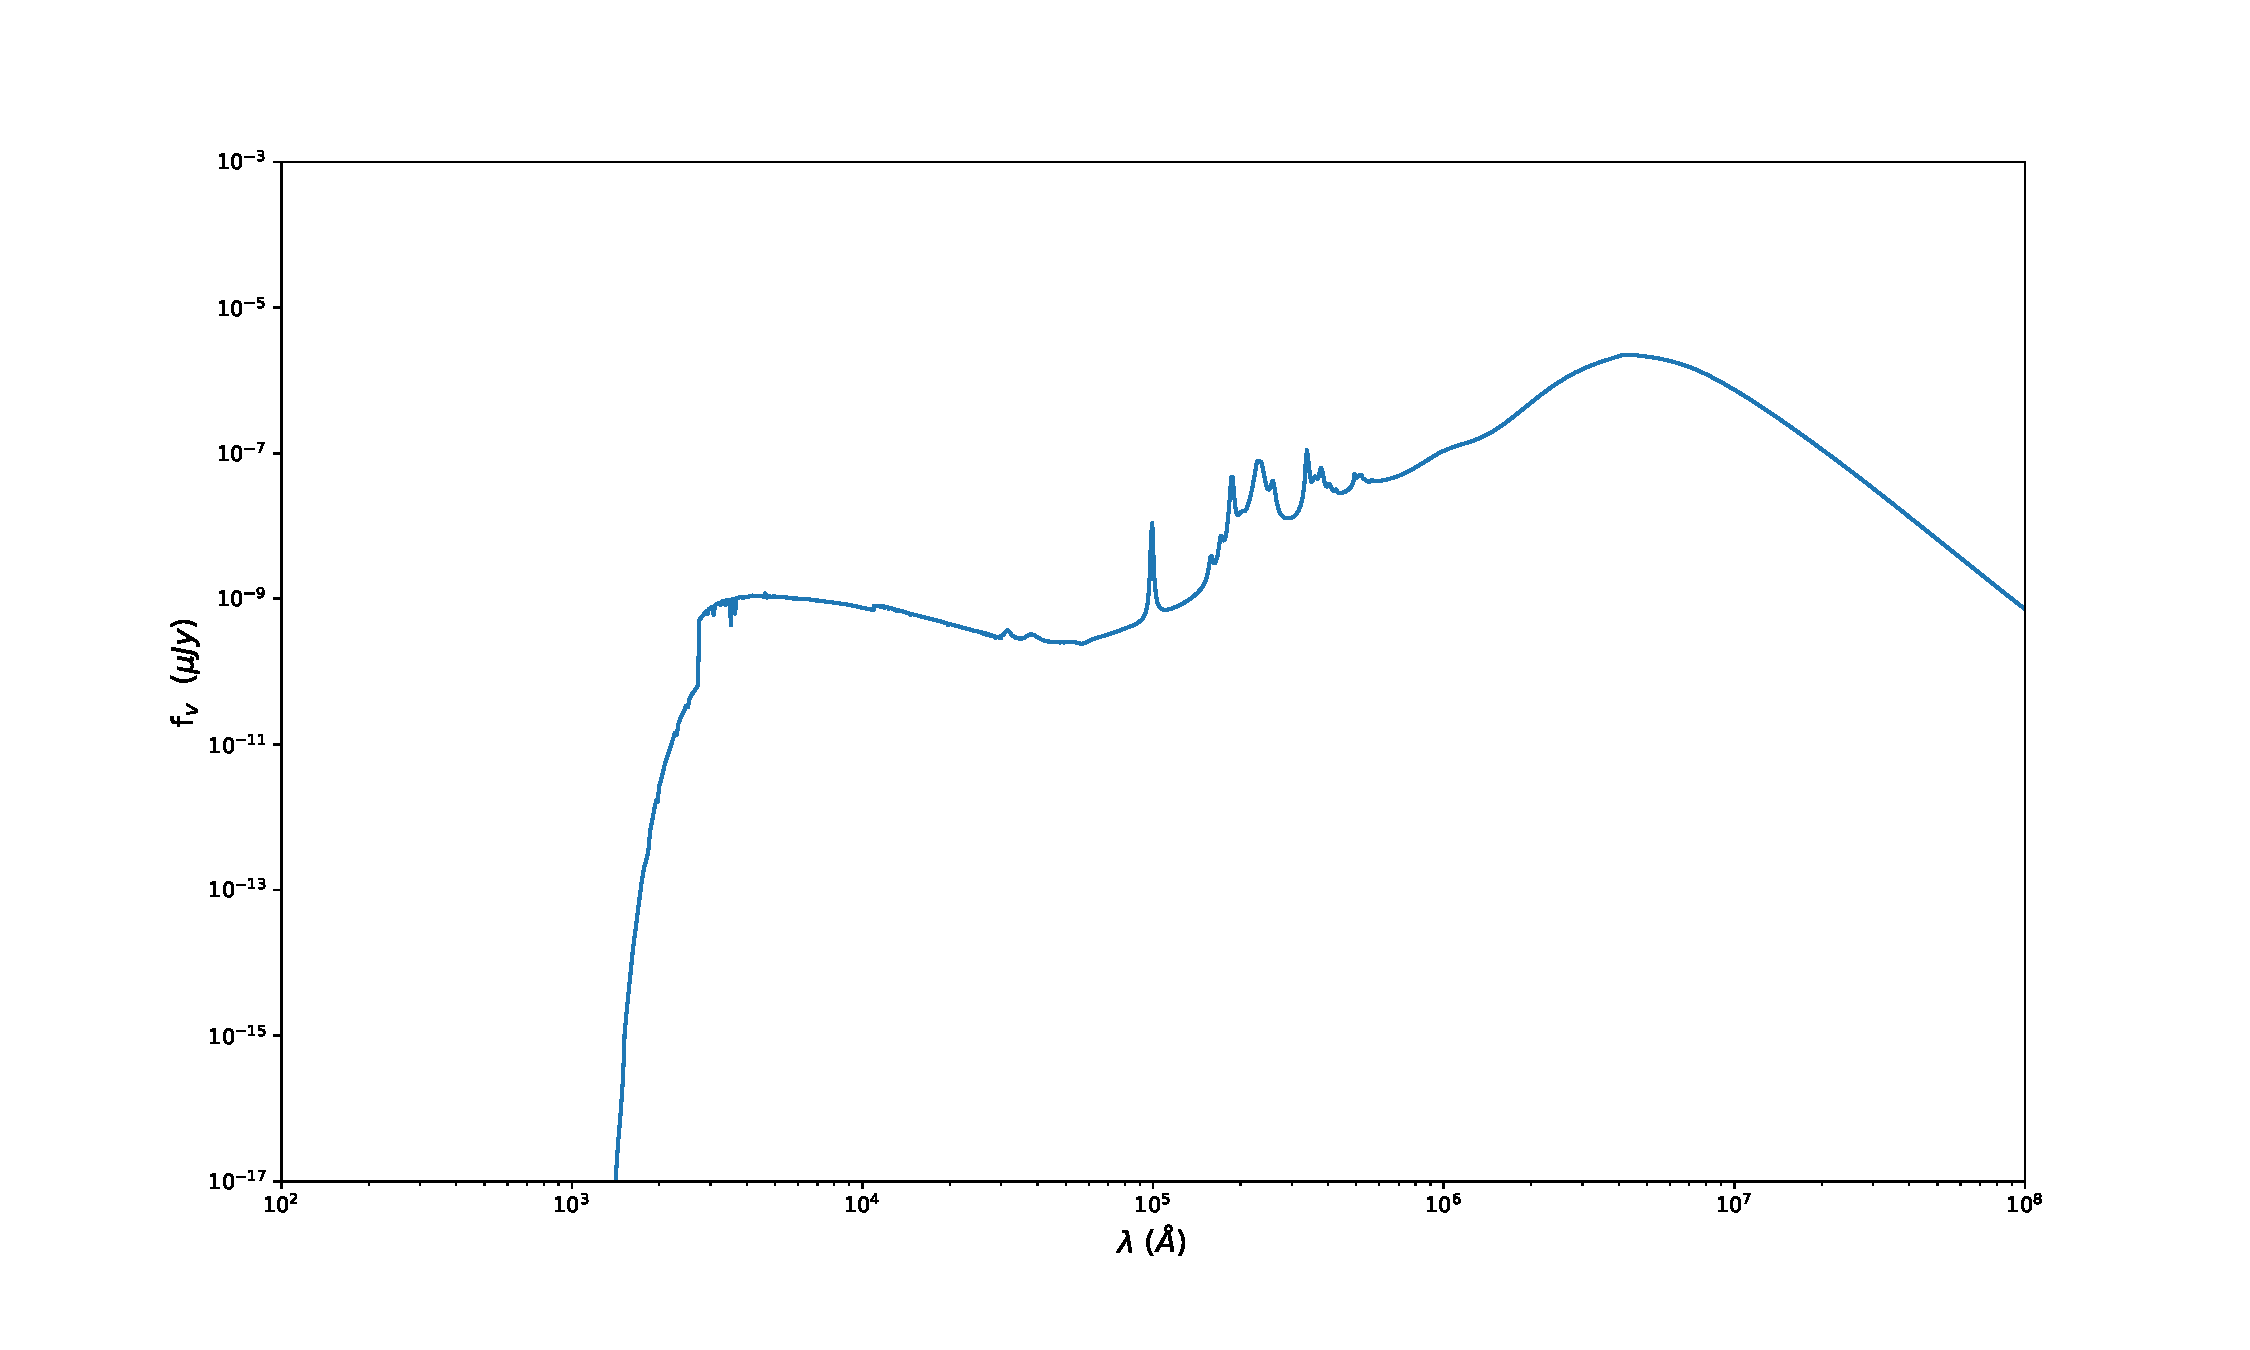
\includegraphics[scale=0.3]{SED redshift 2}
\caption{SED of flux density vs. wavelength at redshift 2}
\end{figure}

\begin{figure}[H]
  \centering
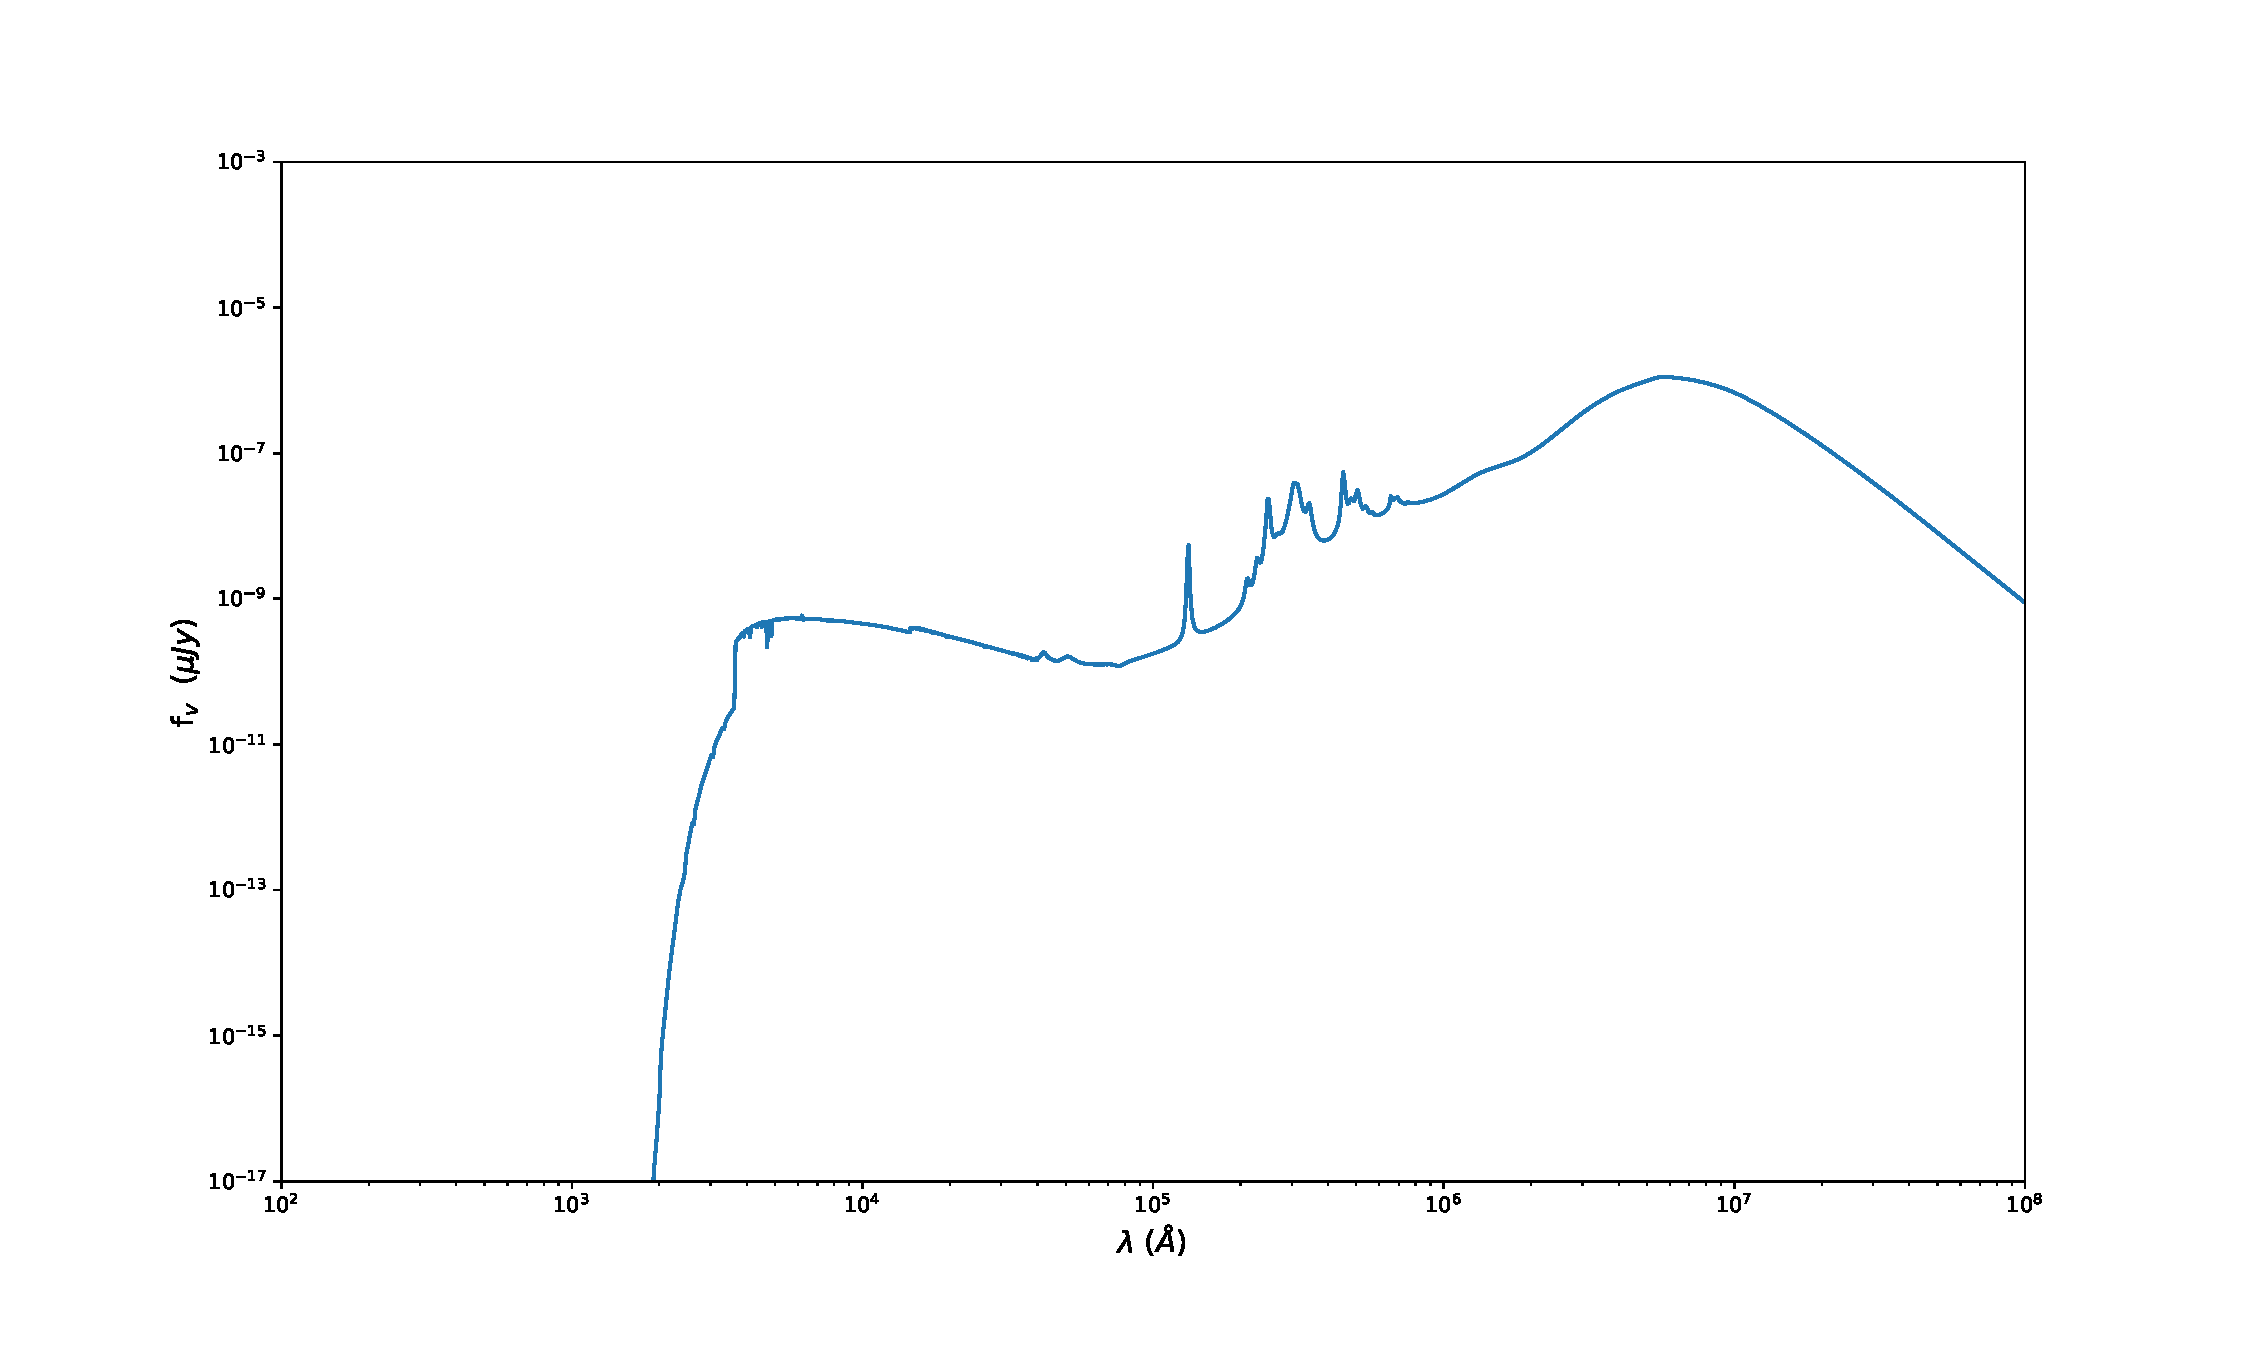
\includegraphics[scale=0.3]{SED redshift 3}
\caption{SED of flux density vs. wavelength at redshift 3}
\end{figure}

Next, the goal was to fix $\lambda = 8000 \AA$ and make a plot of flux density vs. redshift. Note
that at each z the generated SED is not guaranteed to have a flux density value at $\lambda = 8000 \AA$. To
get around this, the wavelength closest to $8000 \AA$ was linearly interpolated to find a reasonable
value for flux density, giving the following graph. As you would expect, flux density decreases as redshift increases.

\begin{figure}[H]
  \centering
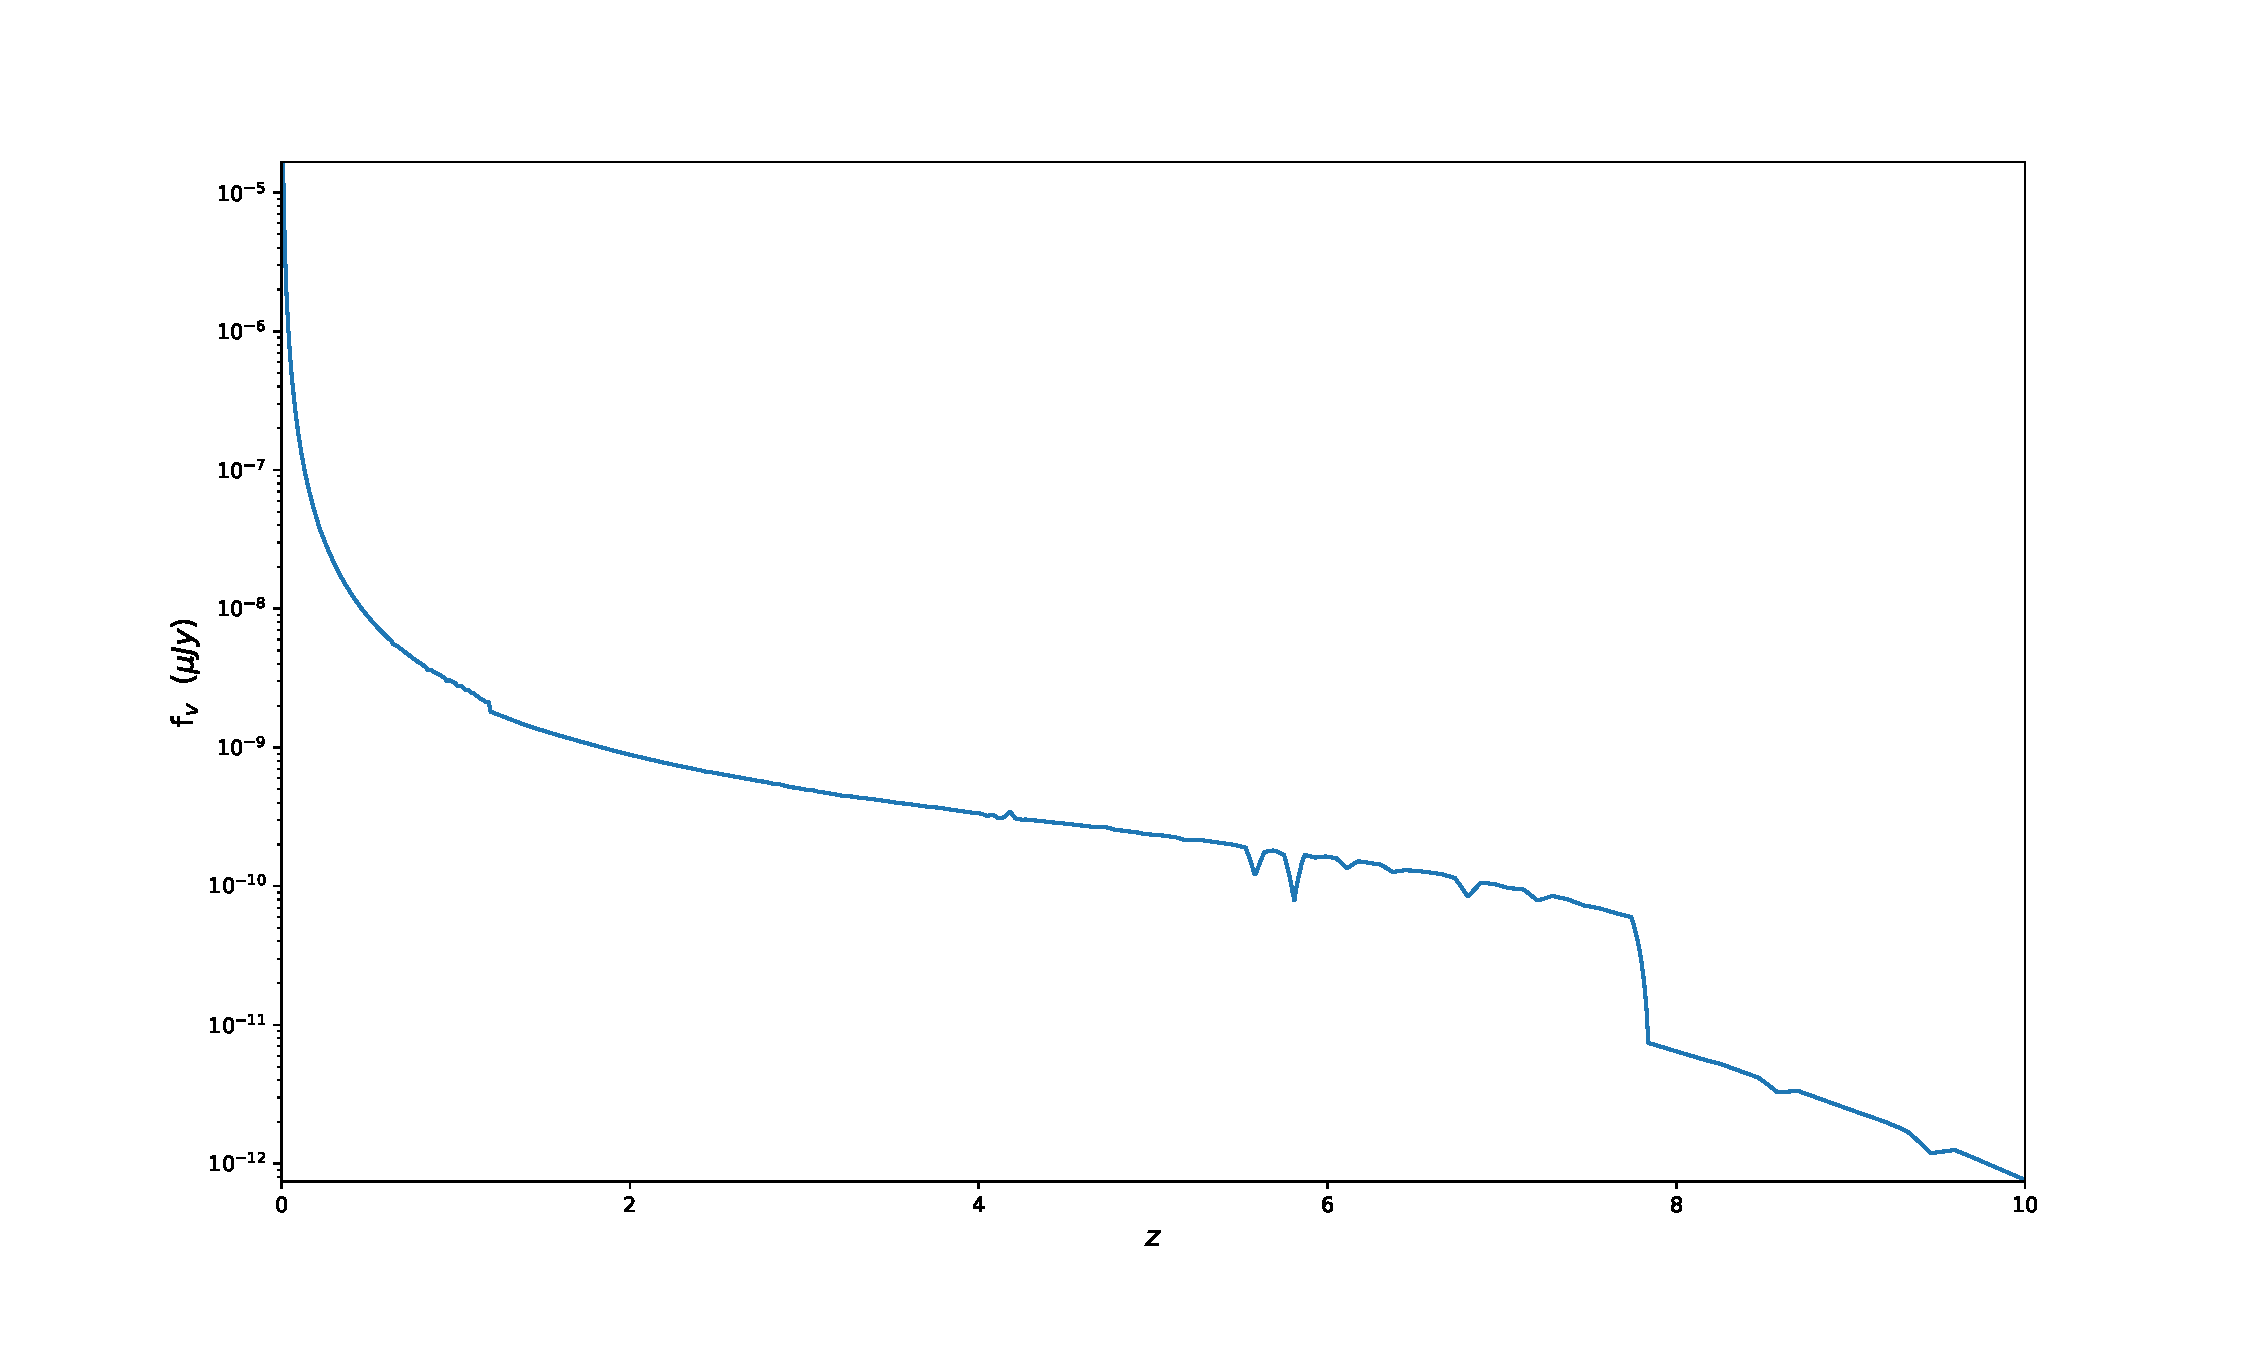
\includegraphics[scale=0.3]{flux density vs redshift}
\caption{Flux density vs. redshift at $\lambda = 8000 \AA$}
\end{figure}

Finally, a function to generate the
SED in flux density ($\mu Jy$) vs. wavelength ($\AA$) for a galaxy
of any age at any redshift was created. Using this function, the following graphs were made.

\begin{figure}[H]
  \centering
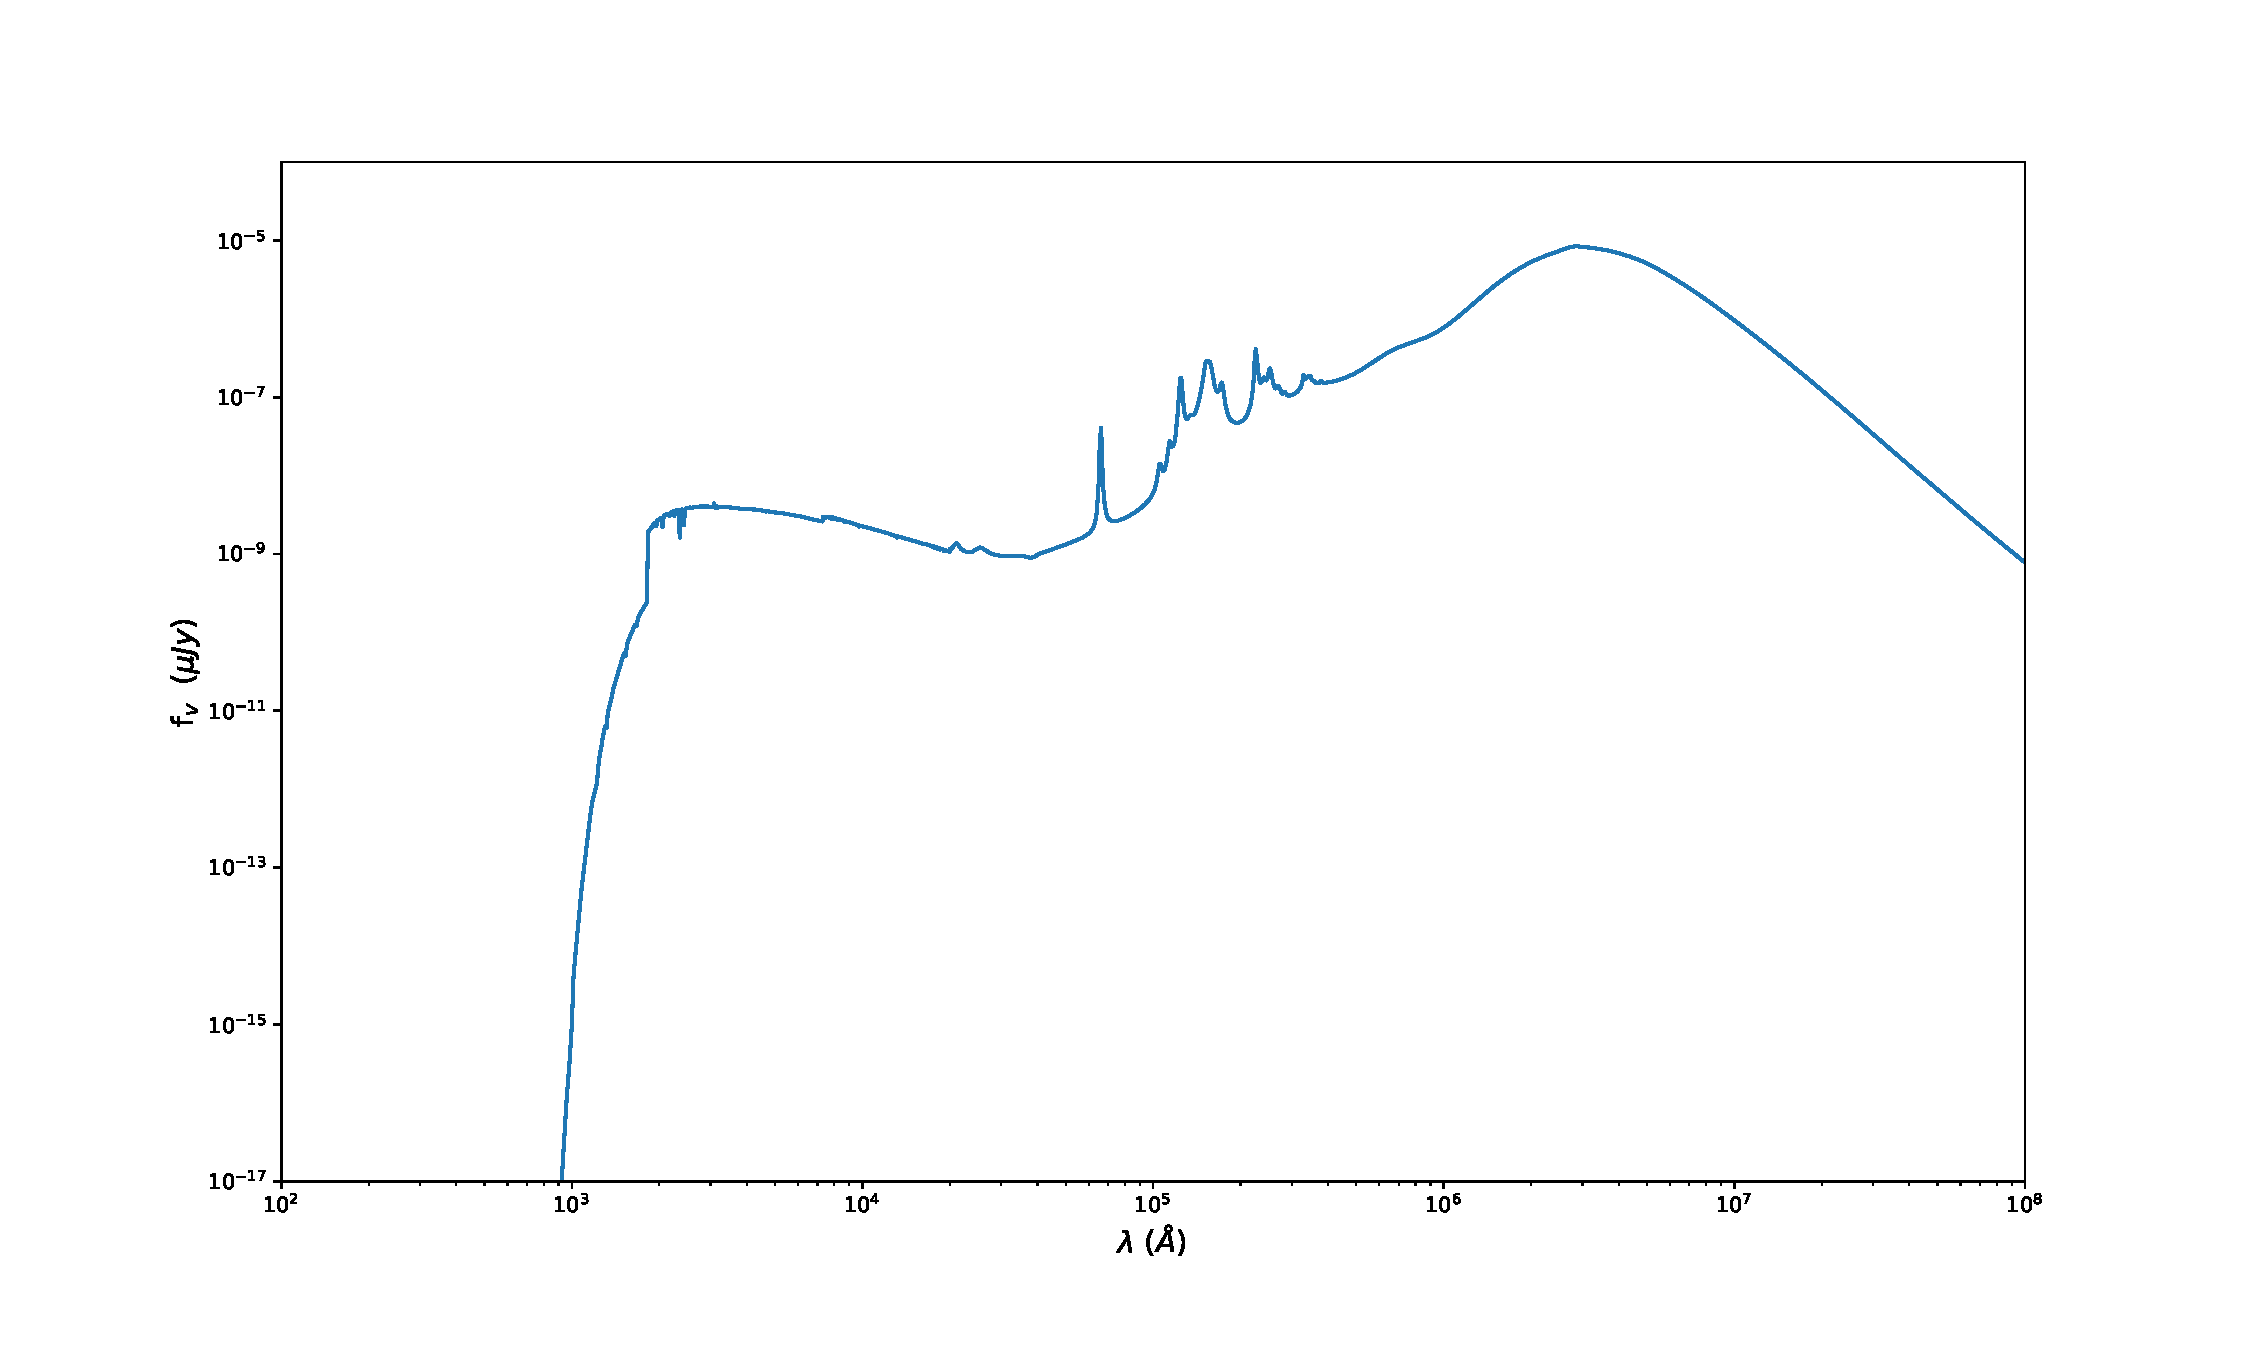
\includegraphics[scale=0.25]{SED age 0.01 redshift 1}
\caption{SED of flux density vs. wavelength for galaxy of age 0.01 Gyr at redshift 1}
\end{figure}

\begin{figure}[H]
  \centering
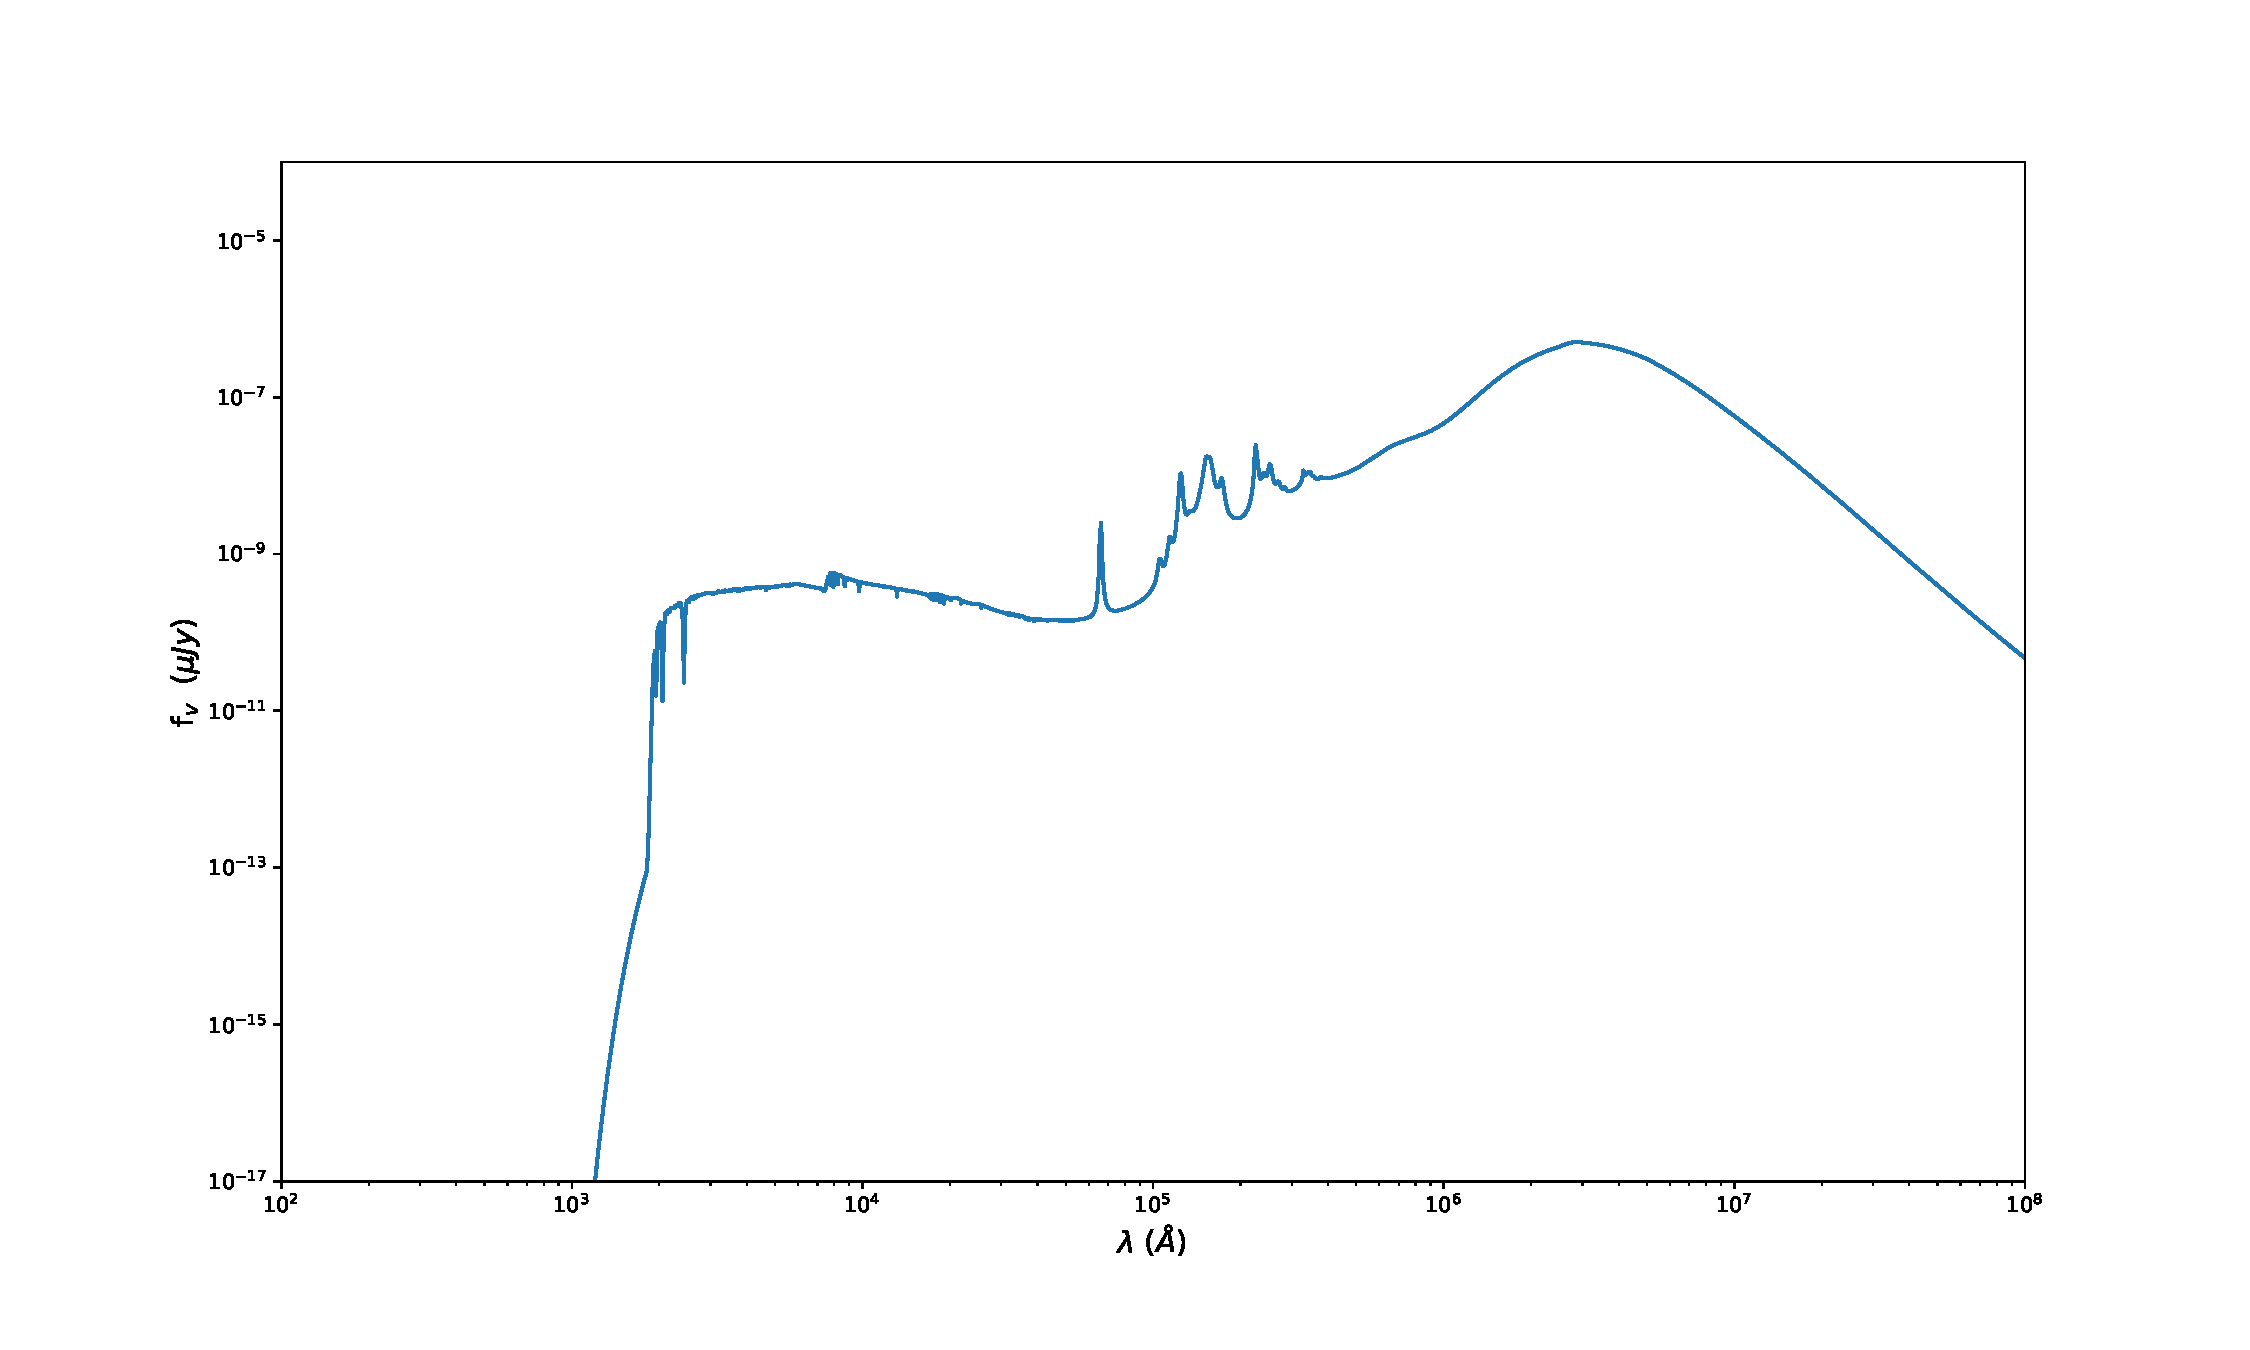
\includegraphics[scale=0.25]{SED age 0.1 redshift 1}
\caption{SED of flux density vs. wavelength for galaxy of age 0.1 Gyr at redshift 1}
\label{fig:9}
\end{figure}

\begin{figure}[H]
  \centering
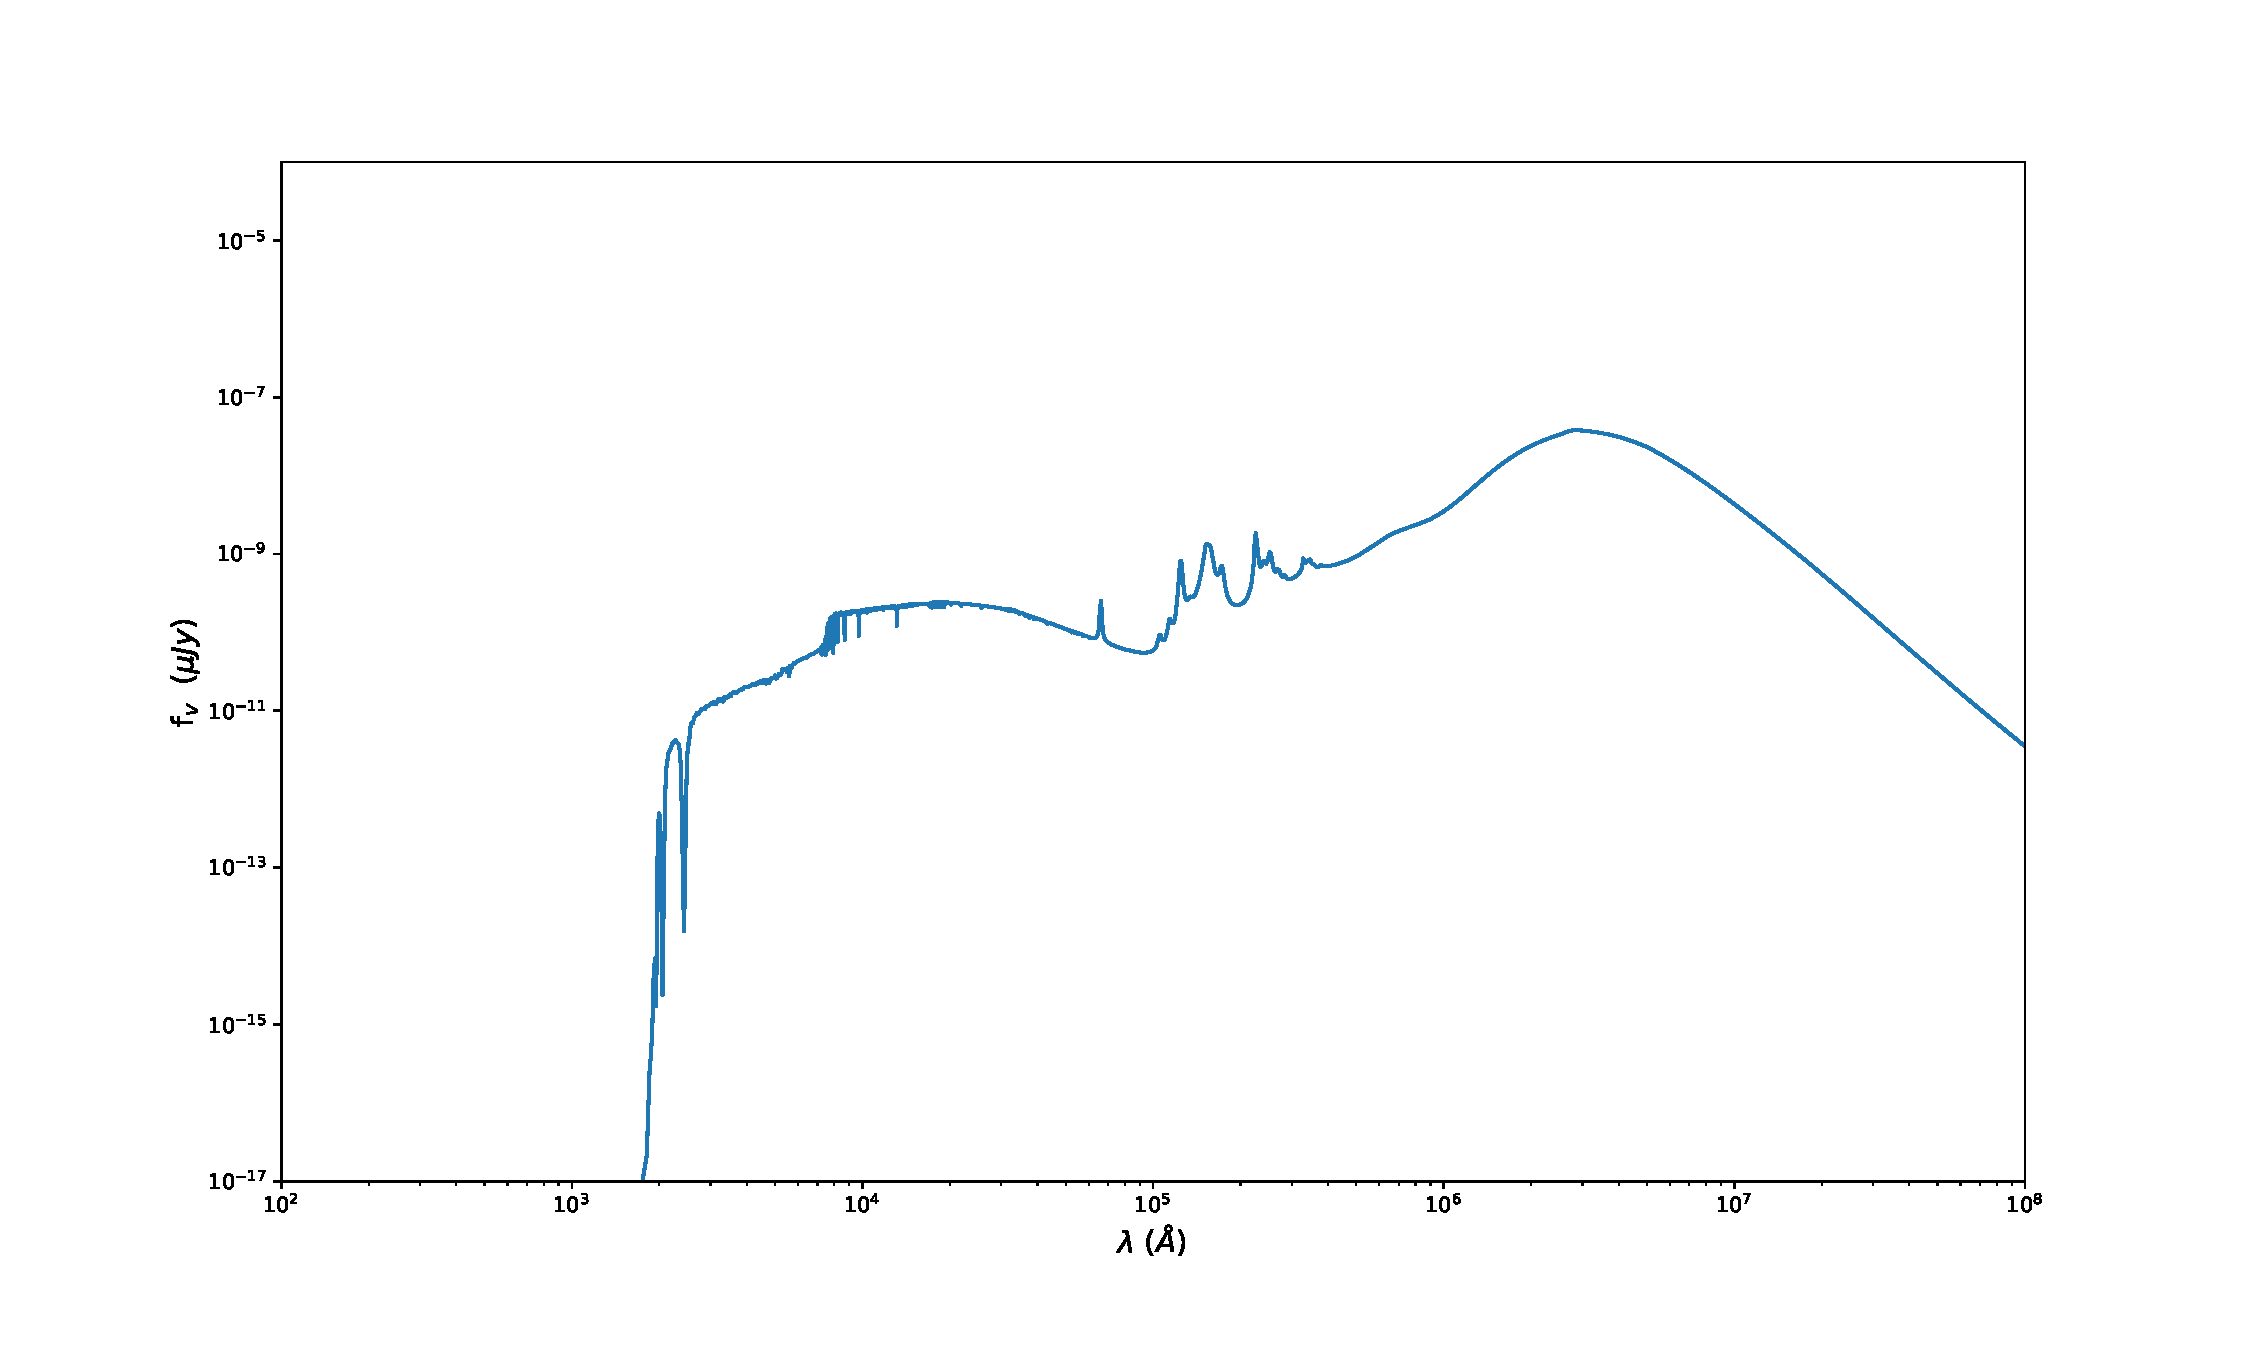
\includegraphics[scale=0.25]{SED age 1 redshift 1}
\caption{SED of flux density vs. wavelength for galaxy of age 1 Gyr at redshift 1}
\end{figure}

\begin{figure}[H]
  \centering
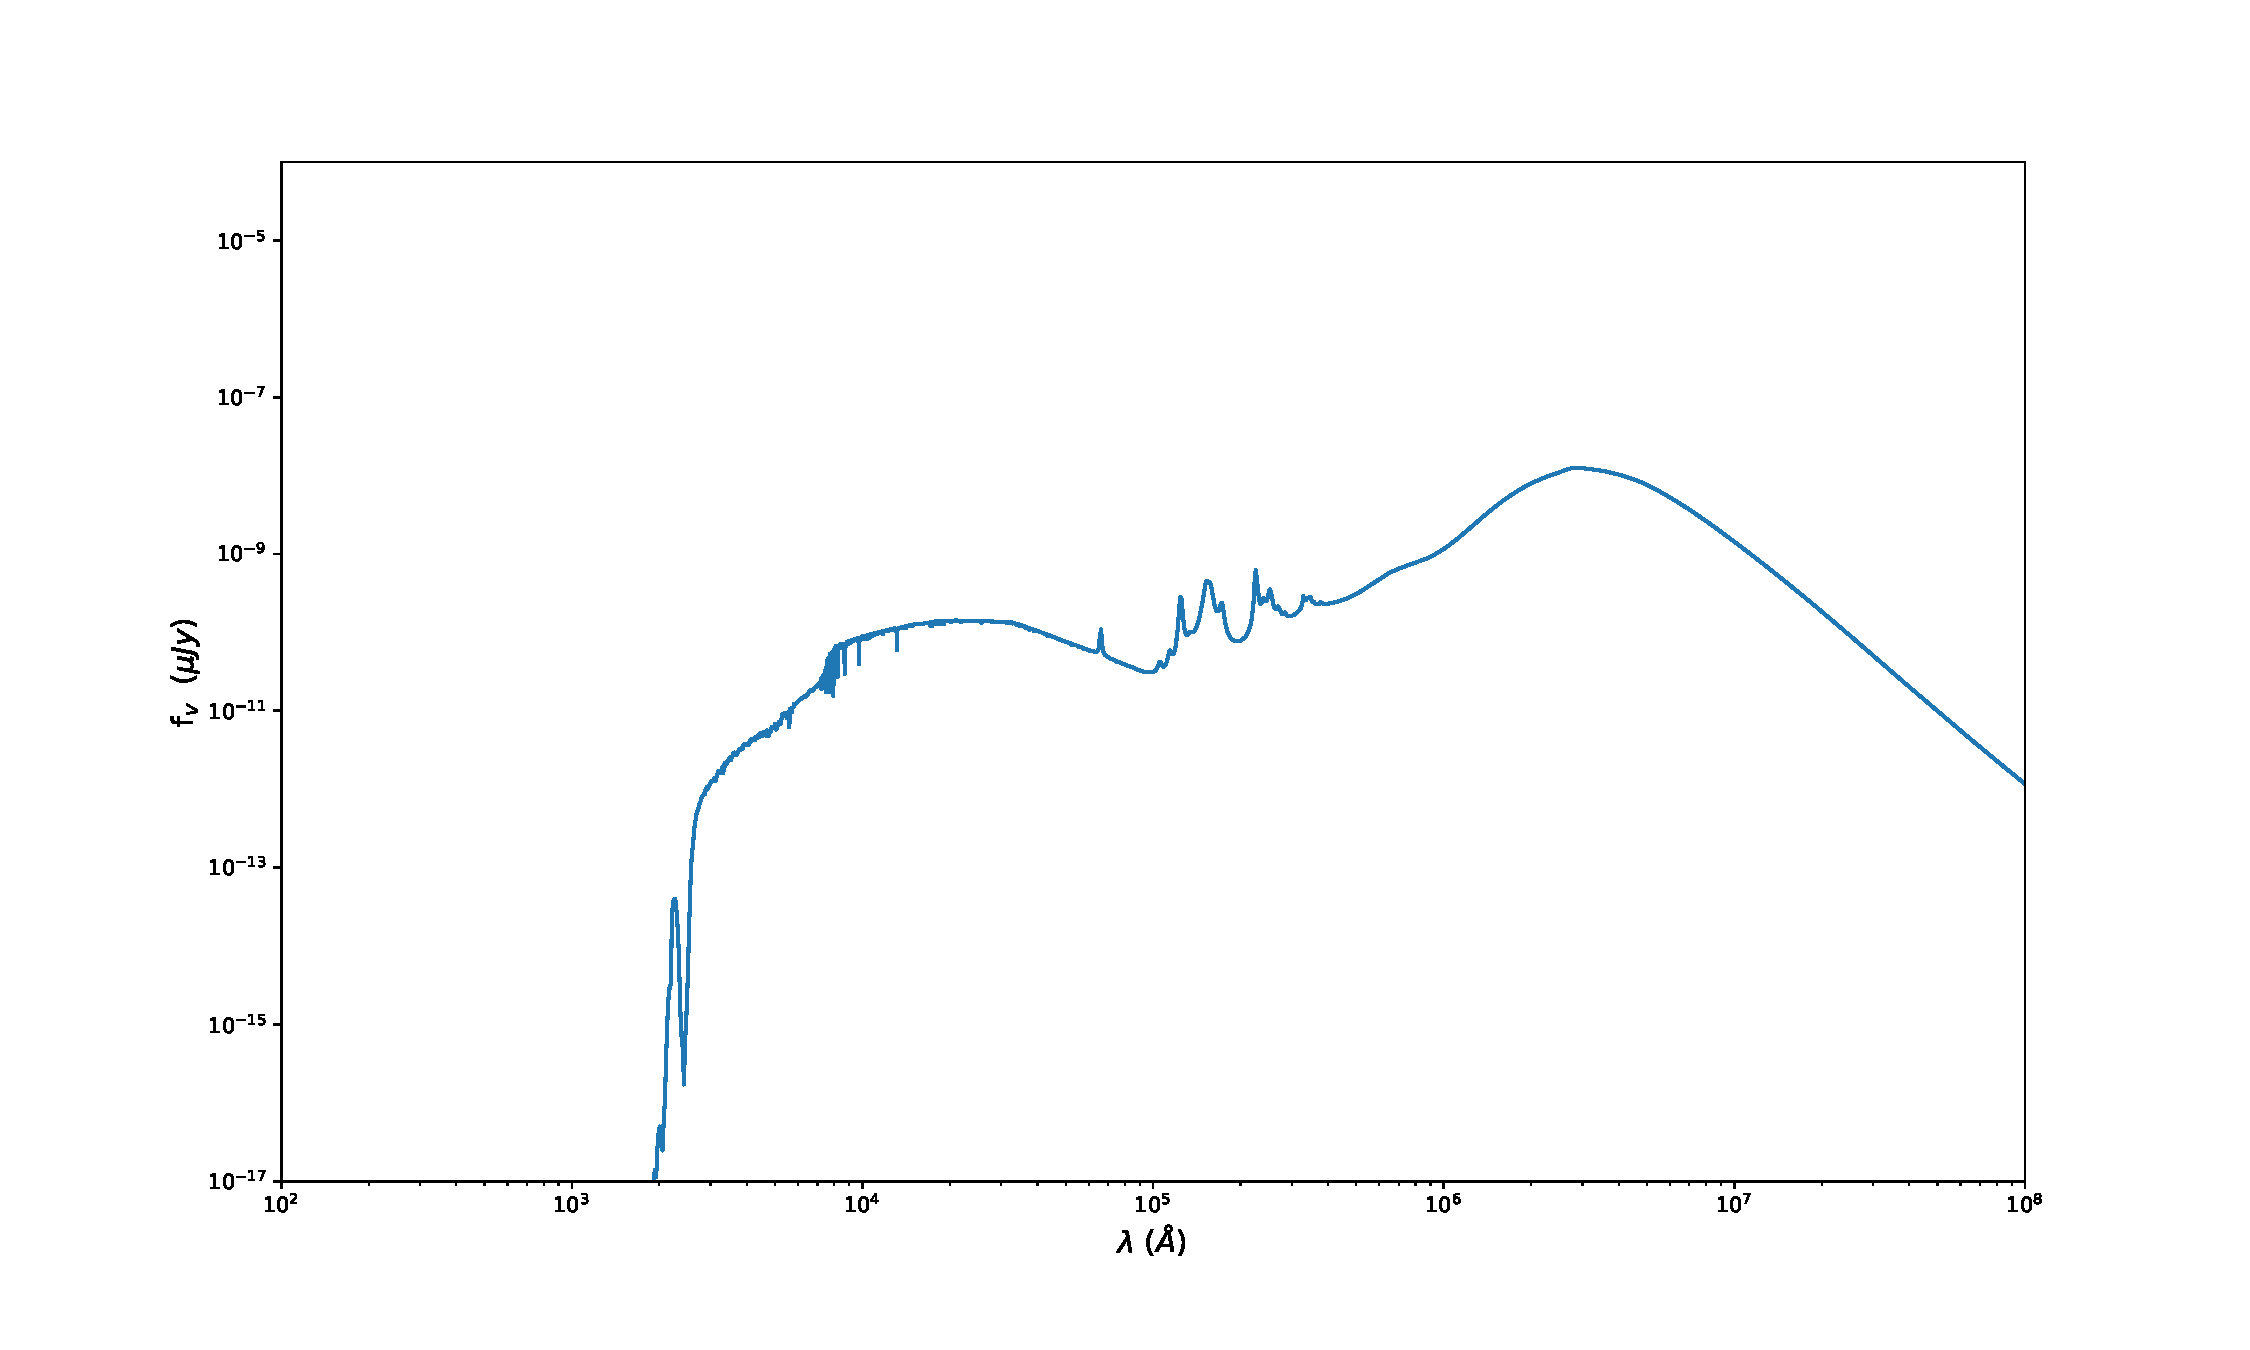
\includegraphics[scale=0.25]{SED age 3 redshift 1}
\caption{SED of flux density vs. wavelength for galaxy of age 3 Gyr at redshift 1}
\end{figure}

\begin{figure}[H]
  \centering
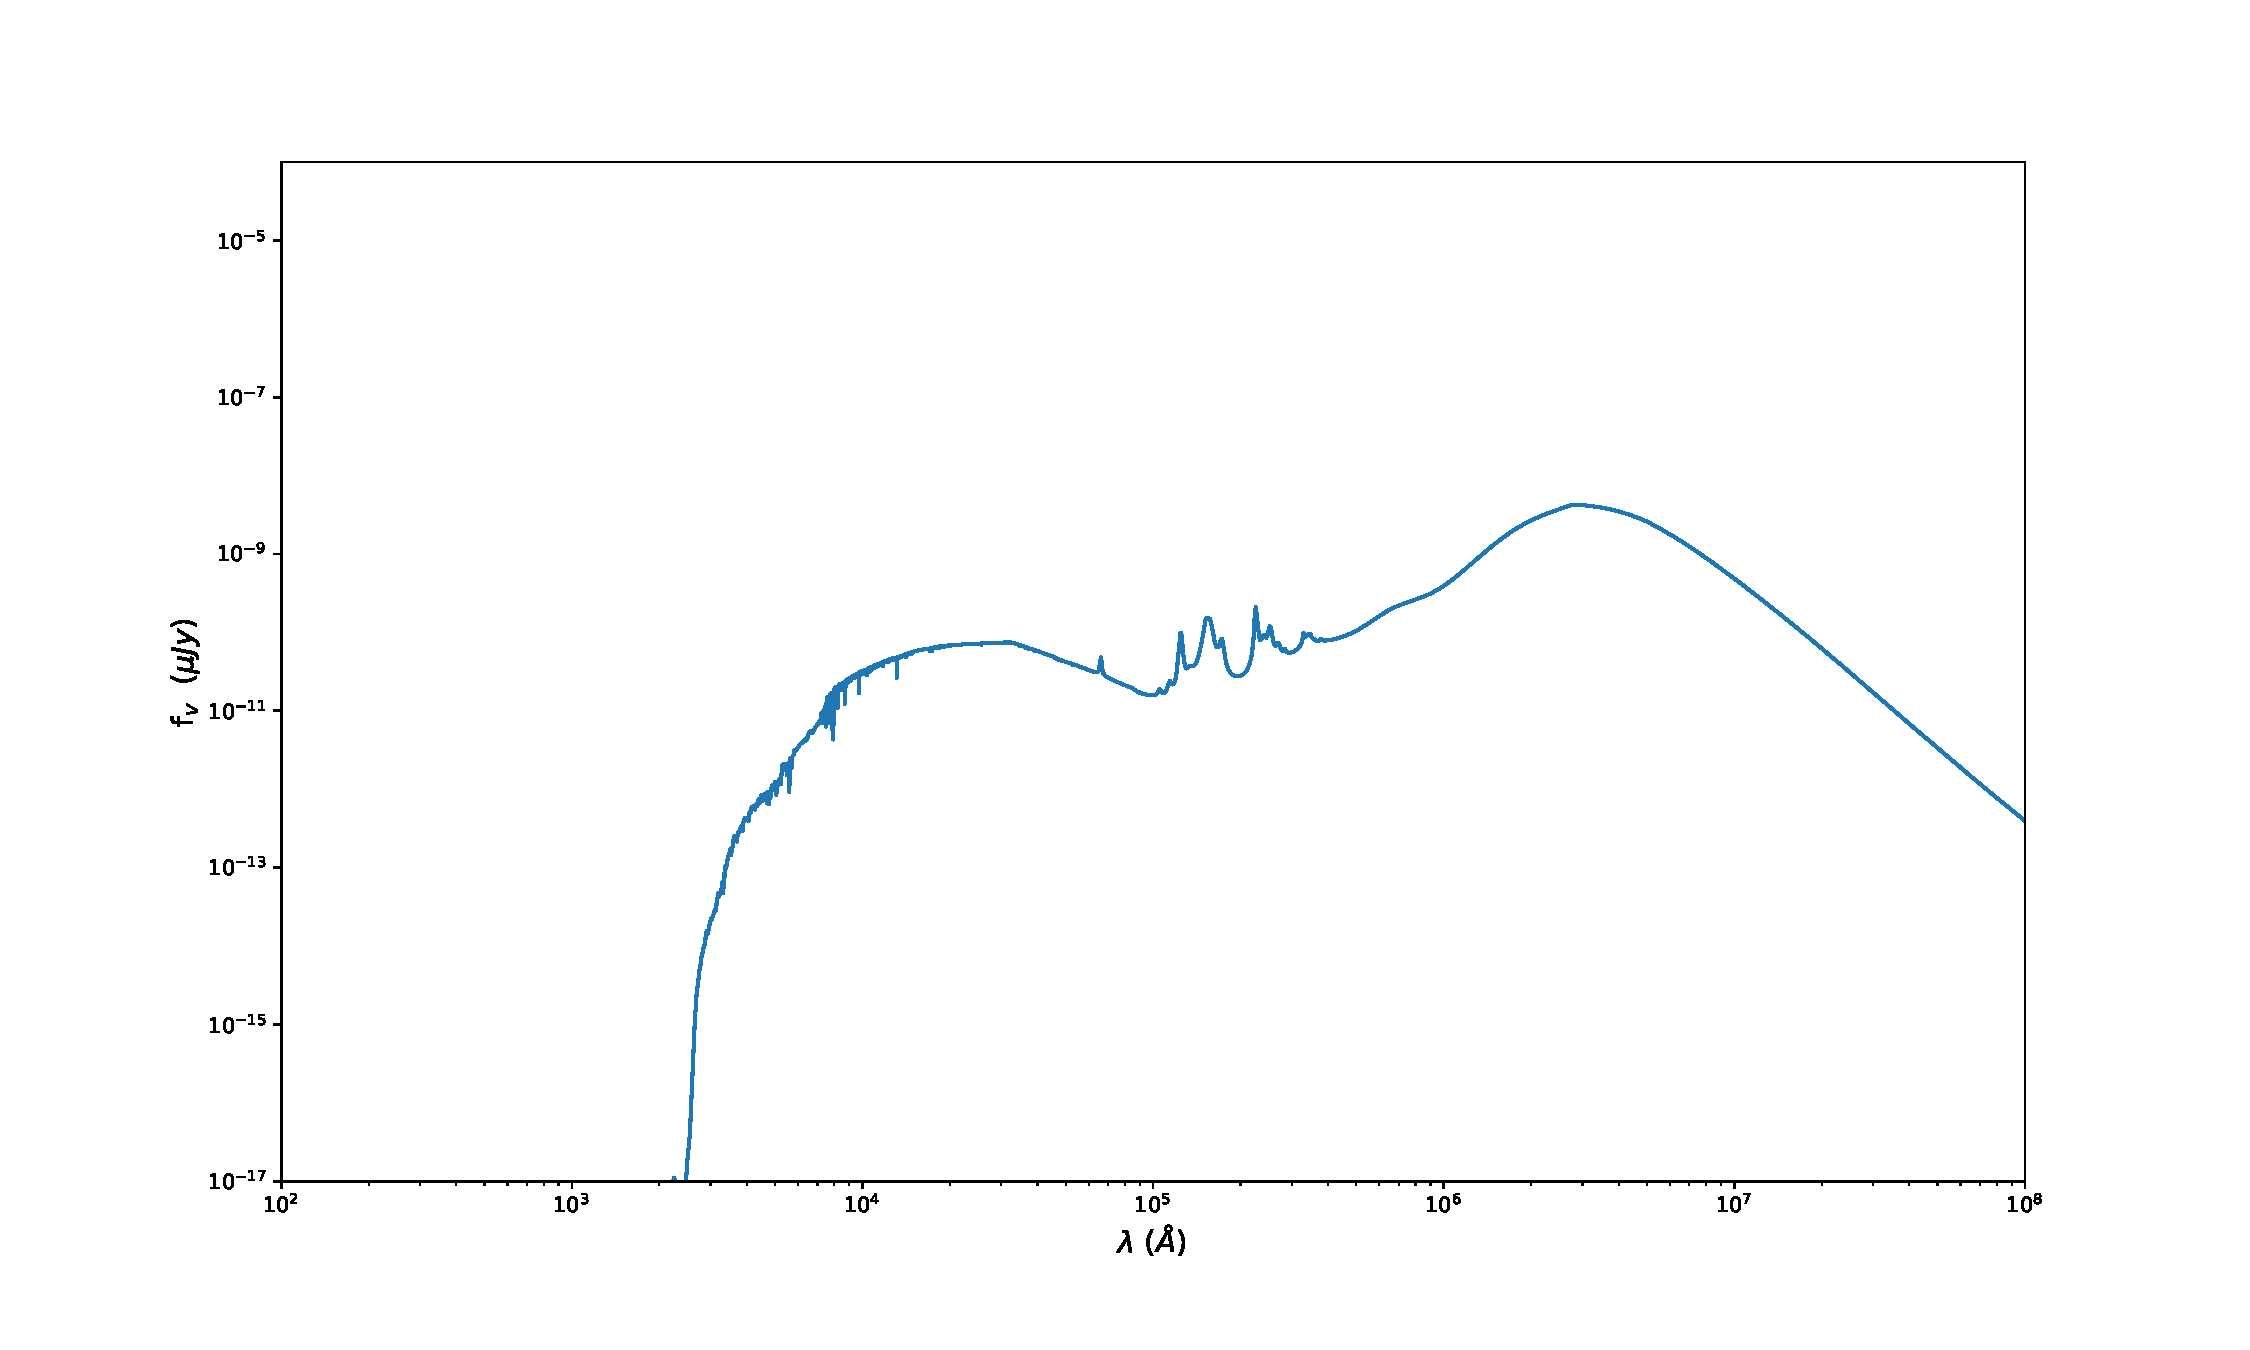
\includegraphics[scale=0.25]{SED age 10 redshift 1}
\caption{SED of flux density vs. wavelength for galaxy of age 10 Gyr at redshift 1}
\end{figure}

\subsection*{Part 2}

In order to fit a straight line to the given data, it was assumed that the error is Gaussian
so that the use of weighted linear least-square fitting is justified (see answer to 2.1 for more motivation). Using linear
algebra, a function to determine the slope and y-intercept (along with uncertainties) was made.
Additionally, a function to calculate $\chi ^2$ was created. Then, the line may be plotted and
its fit may be quantitatively measured.

$$b = -7.390^{+2.158}_{-2.158}$$
$$m = 5.277^{+0.451}_{-0.451}$$

\begin{figure}[H]
  \centering
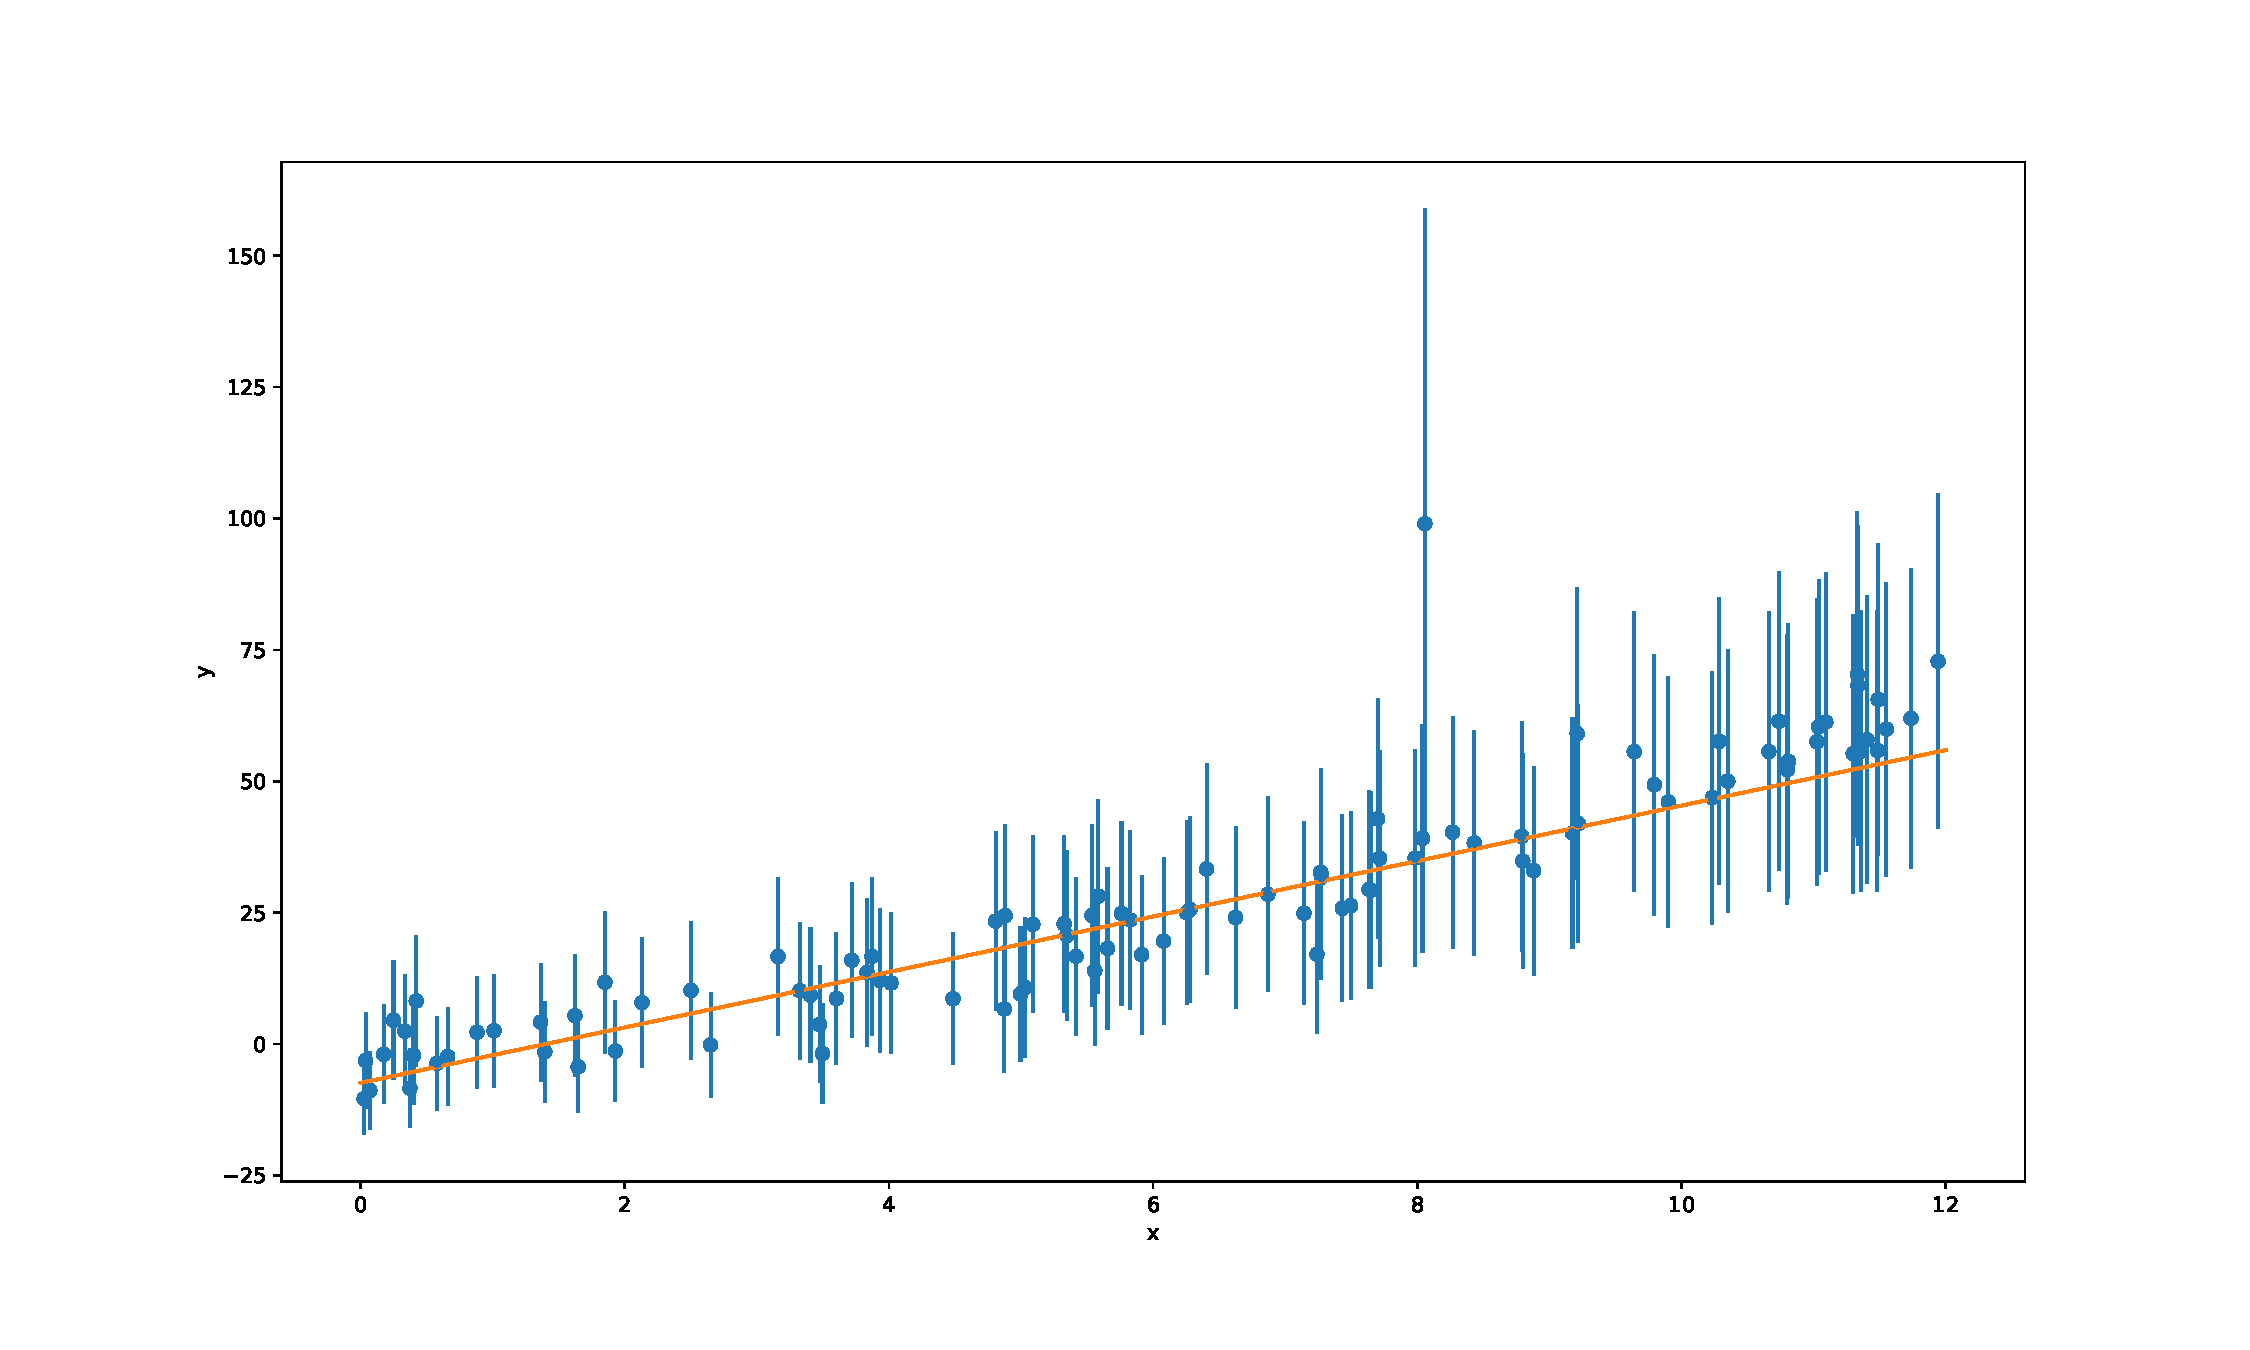
\includegraphics[scale=0.3]{data and line}
\caption{Optimal line to fit the given data. $\chi ^2 = 17,847$}
\end{figure}

Similarily, in order to estimate the age and redshift of the galaxy, we must have a way to quantify
the goodness of fit of a theoretical SED to a noisy observed SED. By the analogy to fitting a
straight line, a similar likelihood function was used:


\begin{figure}[H]
\[Y ^2 = - \sum_{i=1}^{N = 1} \frac{(y_i - f(x_i))^2}{\sigma_{i}^2} \]
\caption{Likelihood function for the fit between theoretical and observational SEDs}
\label{fig:14}
\end{figure}

Where now $y_i$ (Fig.~\ref{fig:14}) represents an observed flux density and $f(x_i)$ is the theoretical flux density.
Note that the negative sign is required because a higher likelihood must imply a closer fit. With
this definition in place, we can now compare how a galaxy with age 0.1 Gyr at z = 1.0 compares with
galaxy 1 and galaxy 2's SEDs. This galaxy had a likelihood of -3121221711061.225 with galaxy 1 and a
likelihood of -364732.5275292772 with galaxy 2.

\begin{figure}[H]
  \centering
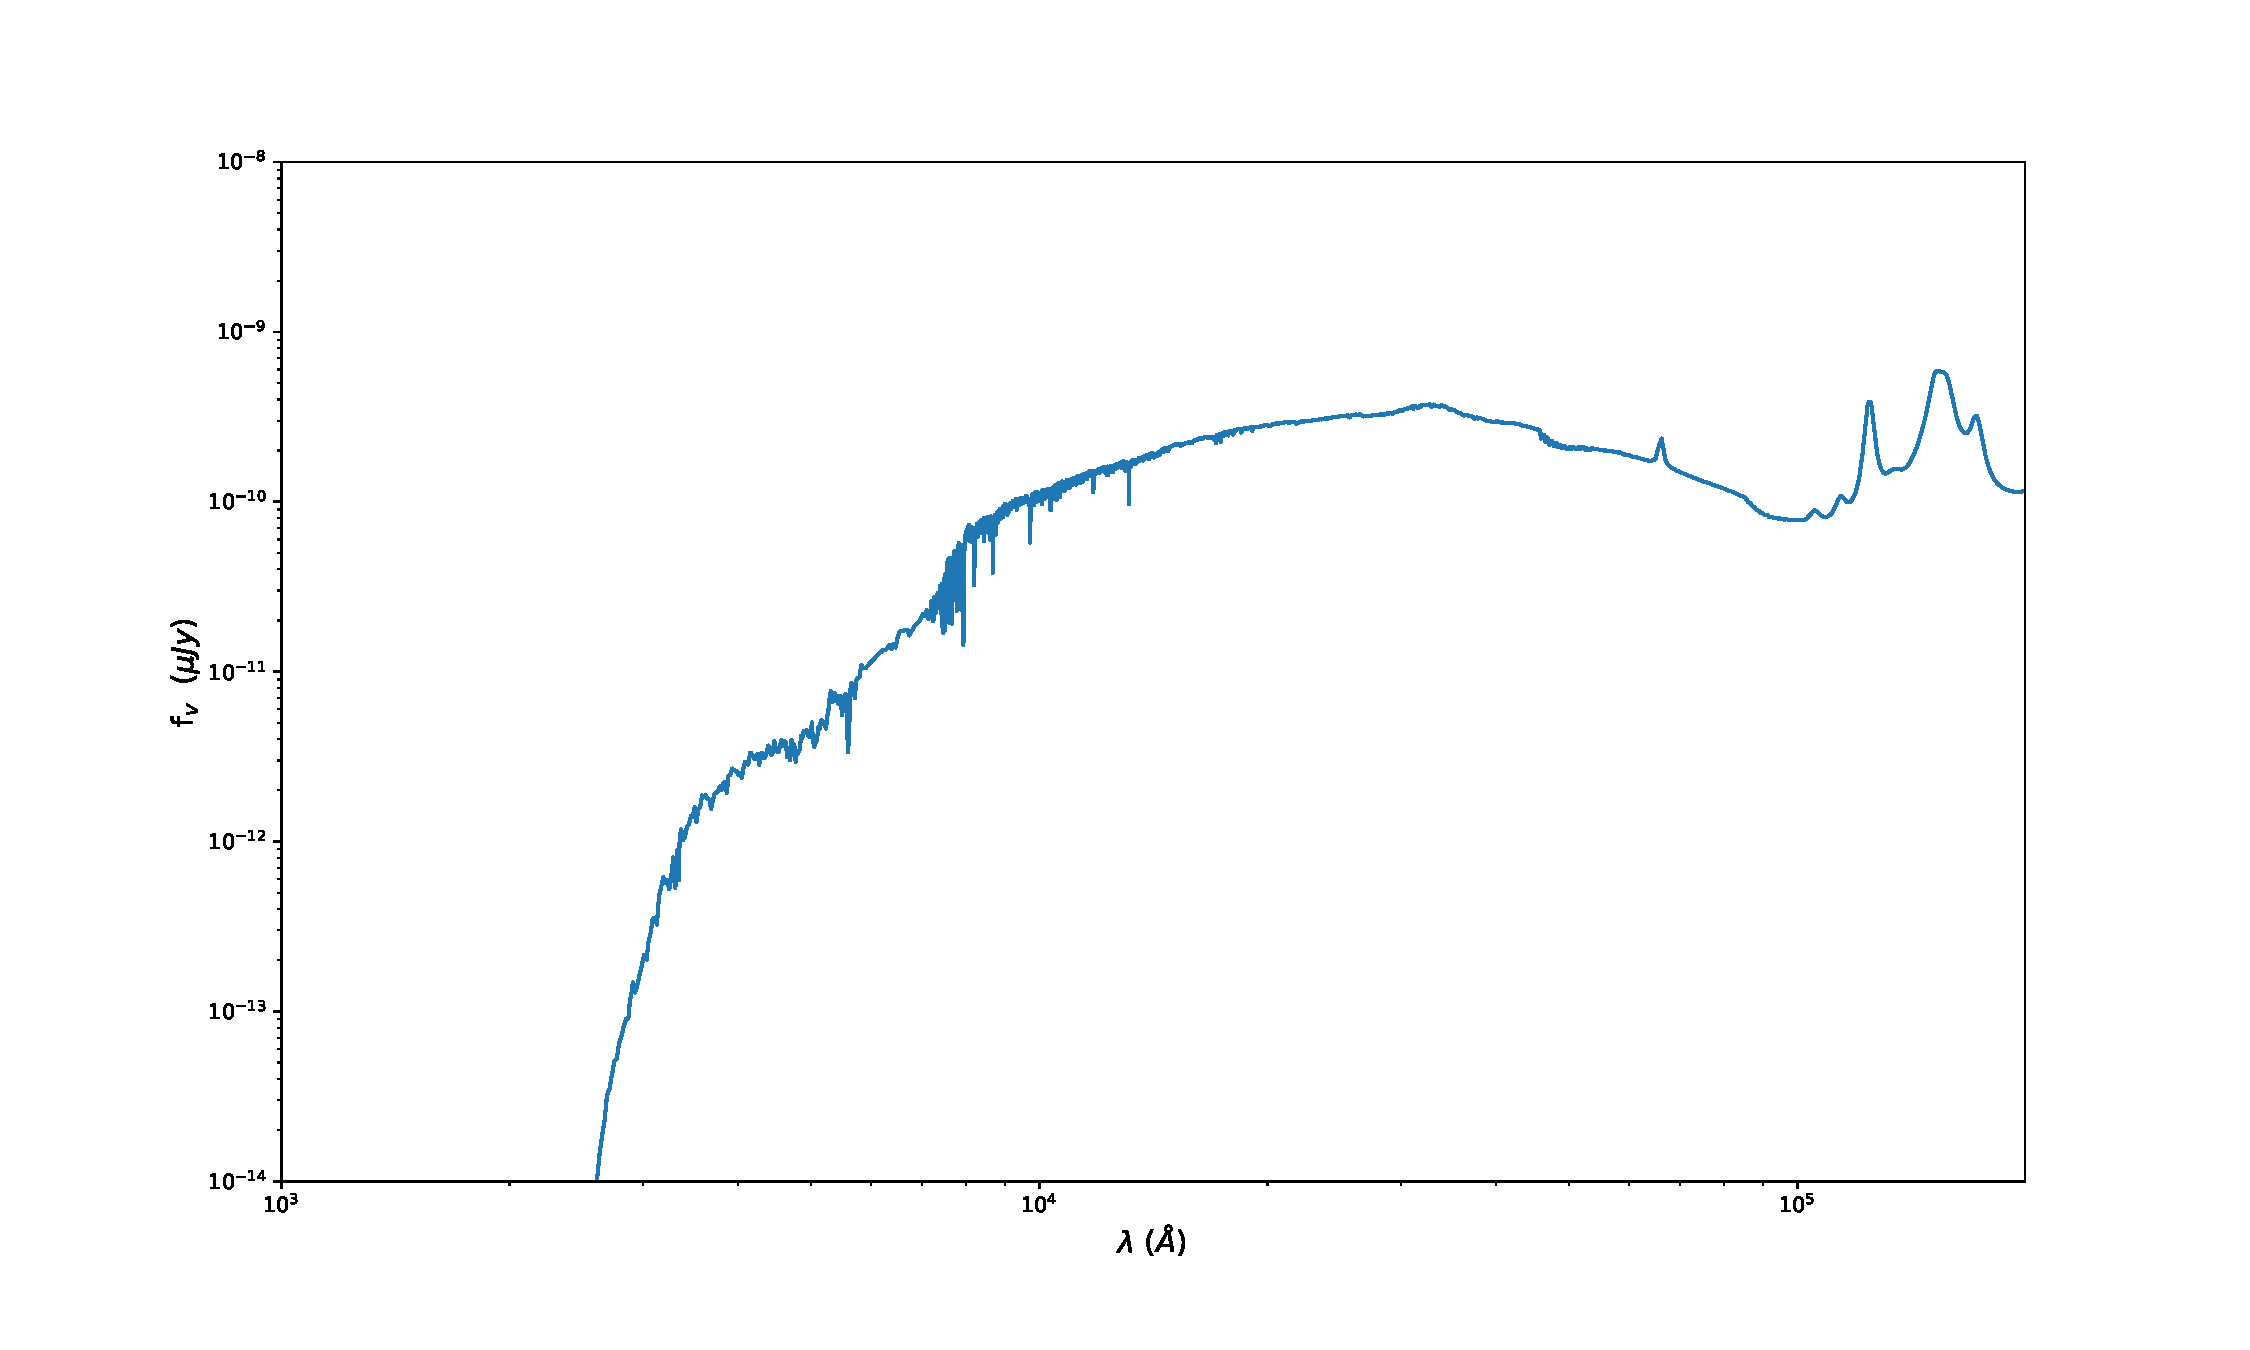
\includegraphics[scale=0.25]{SED galaxy 1}
\caption{given SED of galaxy 1}
\end{figure}

\begin{figure}[H]
  \centering
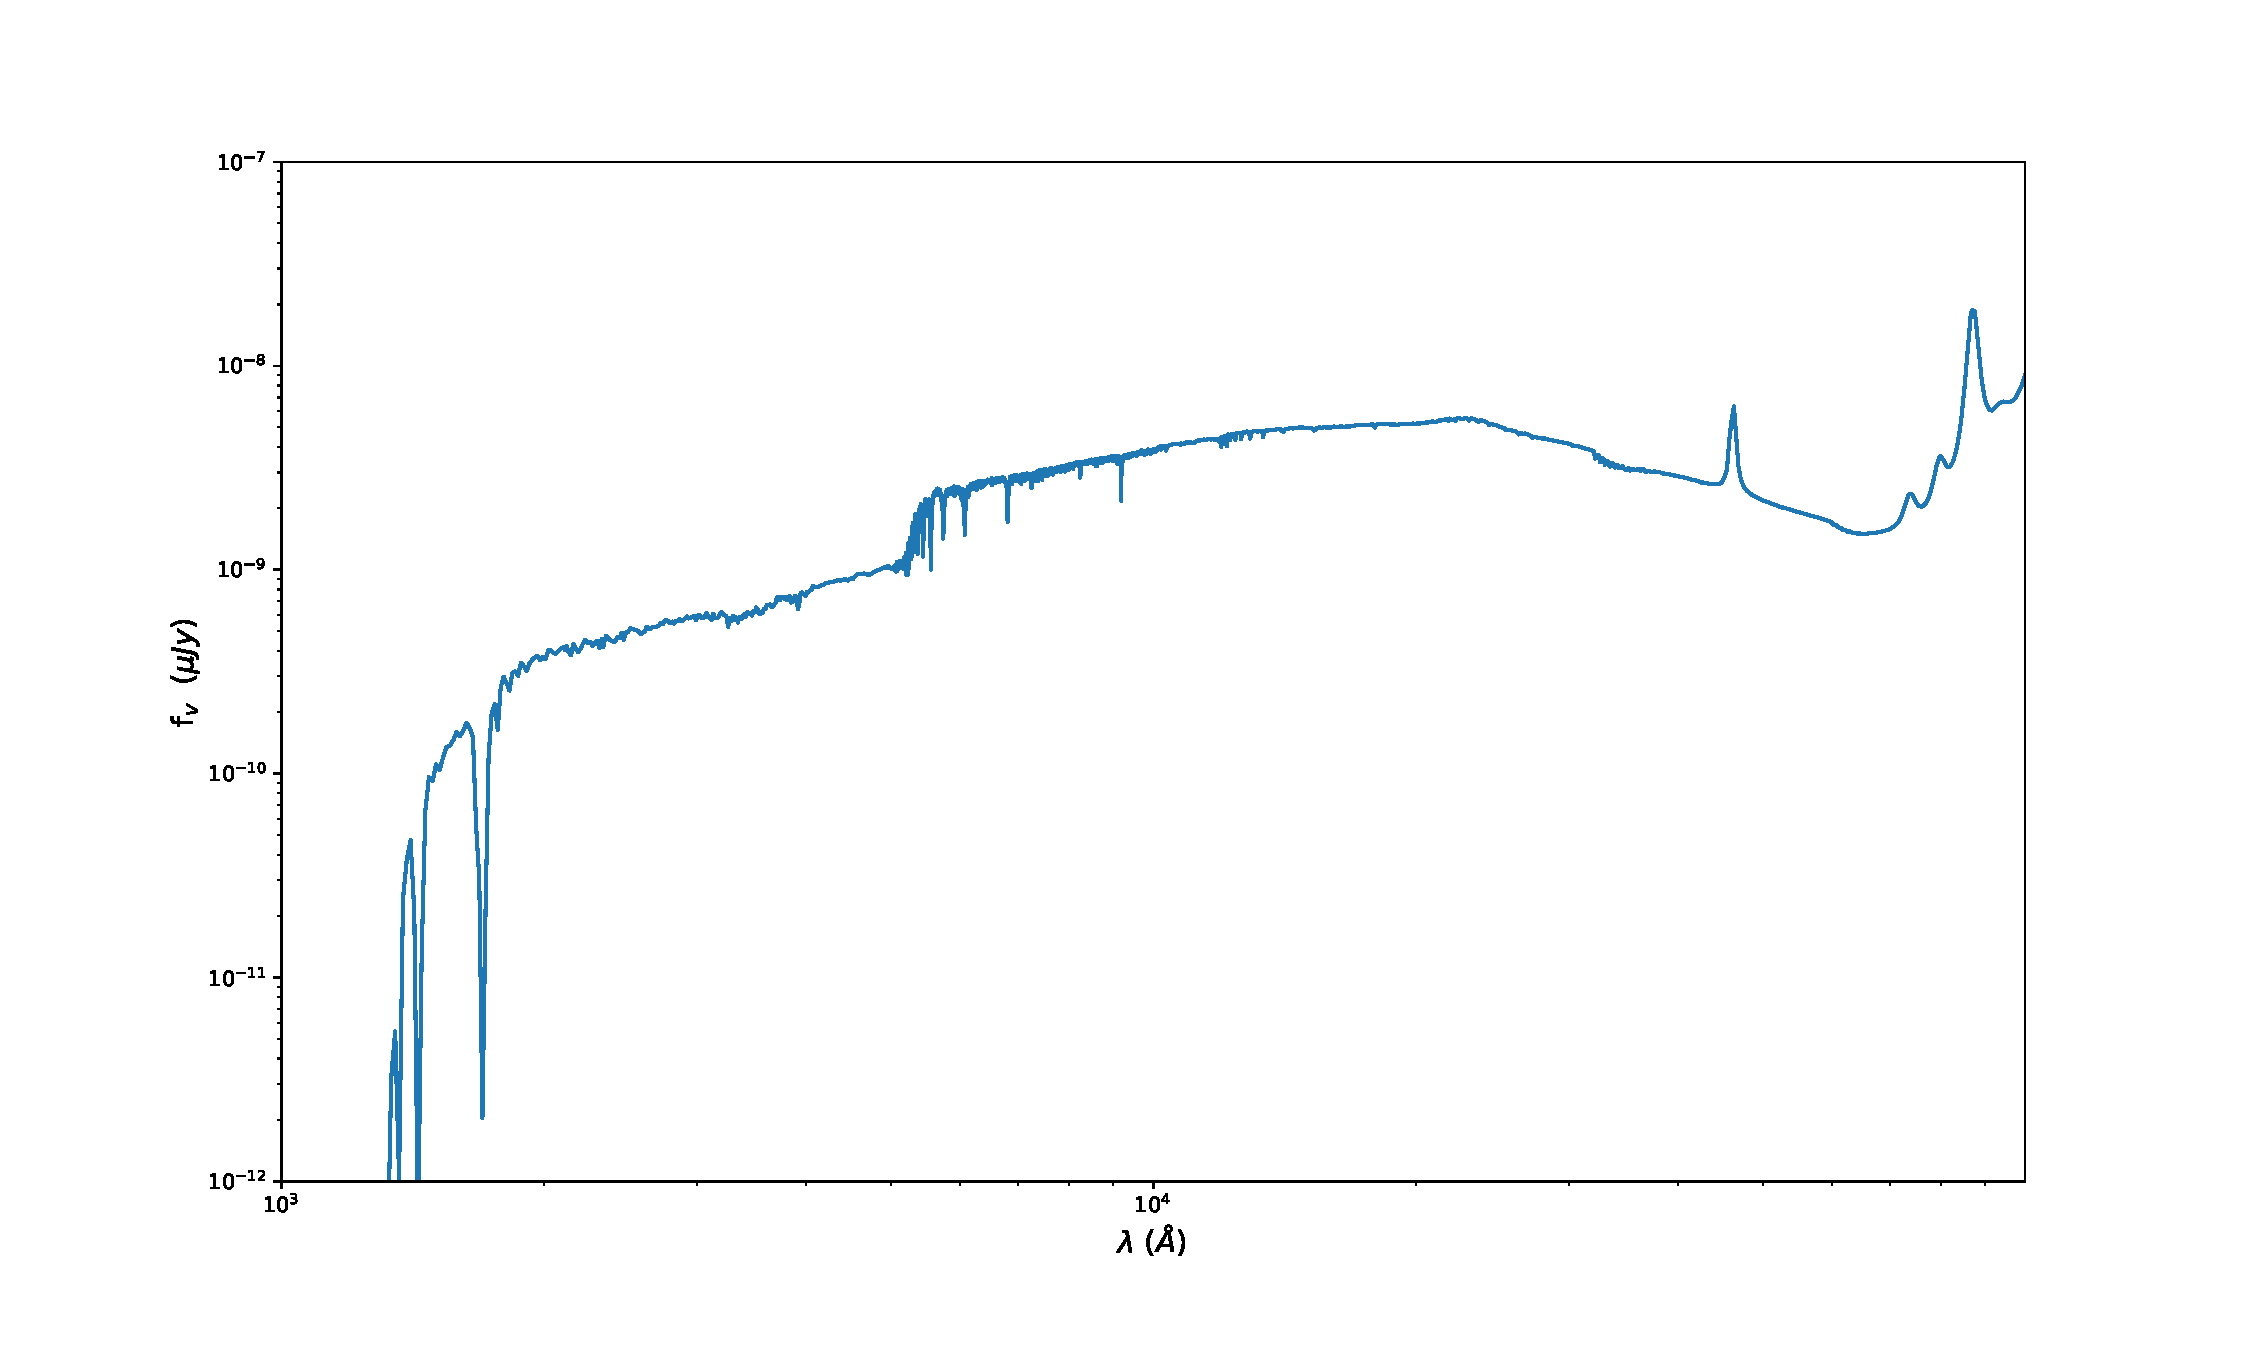
\includegraphics[scale=0.25]{SED galaxy 2}
\caption{given SED of galaxy 2}
\end{figure}

%Include figure
Clearly, a galaxy with age 0.1 Gyr (Fig.~\ref{fig:9}) and z = 1.0 has a more similar SED to galaxy 2, which makes sense
when comparing the SED of galaxy 2 to the SED of this galaxy (above, include figure). By using the
likelihood function, we may also try to brute force our way to an estimate of the proper age and z
of these galaxies. That is, we may loop through a number of combinations of age and z to find which combination
has the highest likelihood. Using this implemented function, we get that galaxy 1 has age of around
6.4 Gyr and redshift of 0.8 and galaxy 2 has age of around 3.4 Gyr and redshift 0.2.


\begin{figure}[H]
  \centering
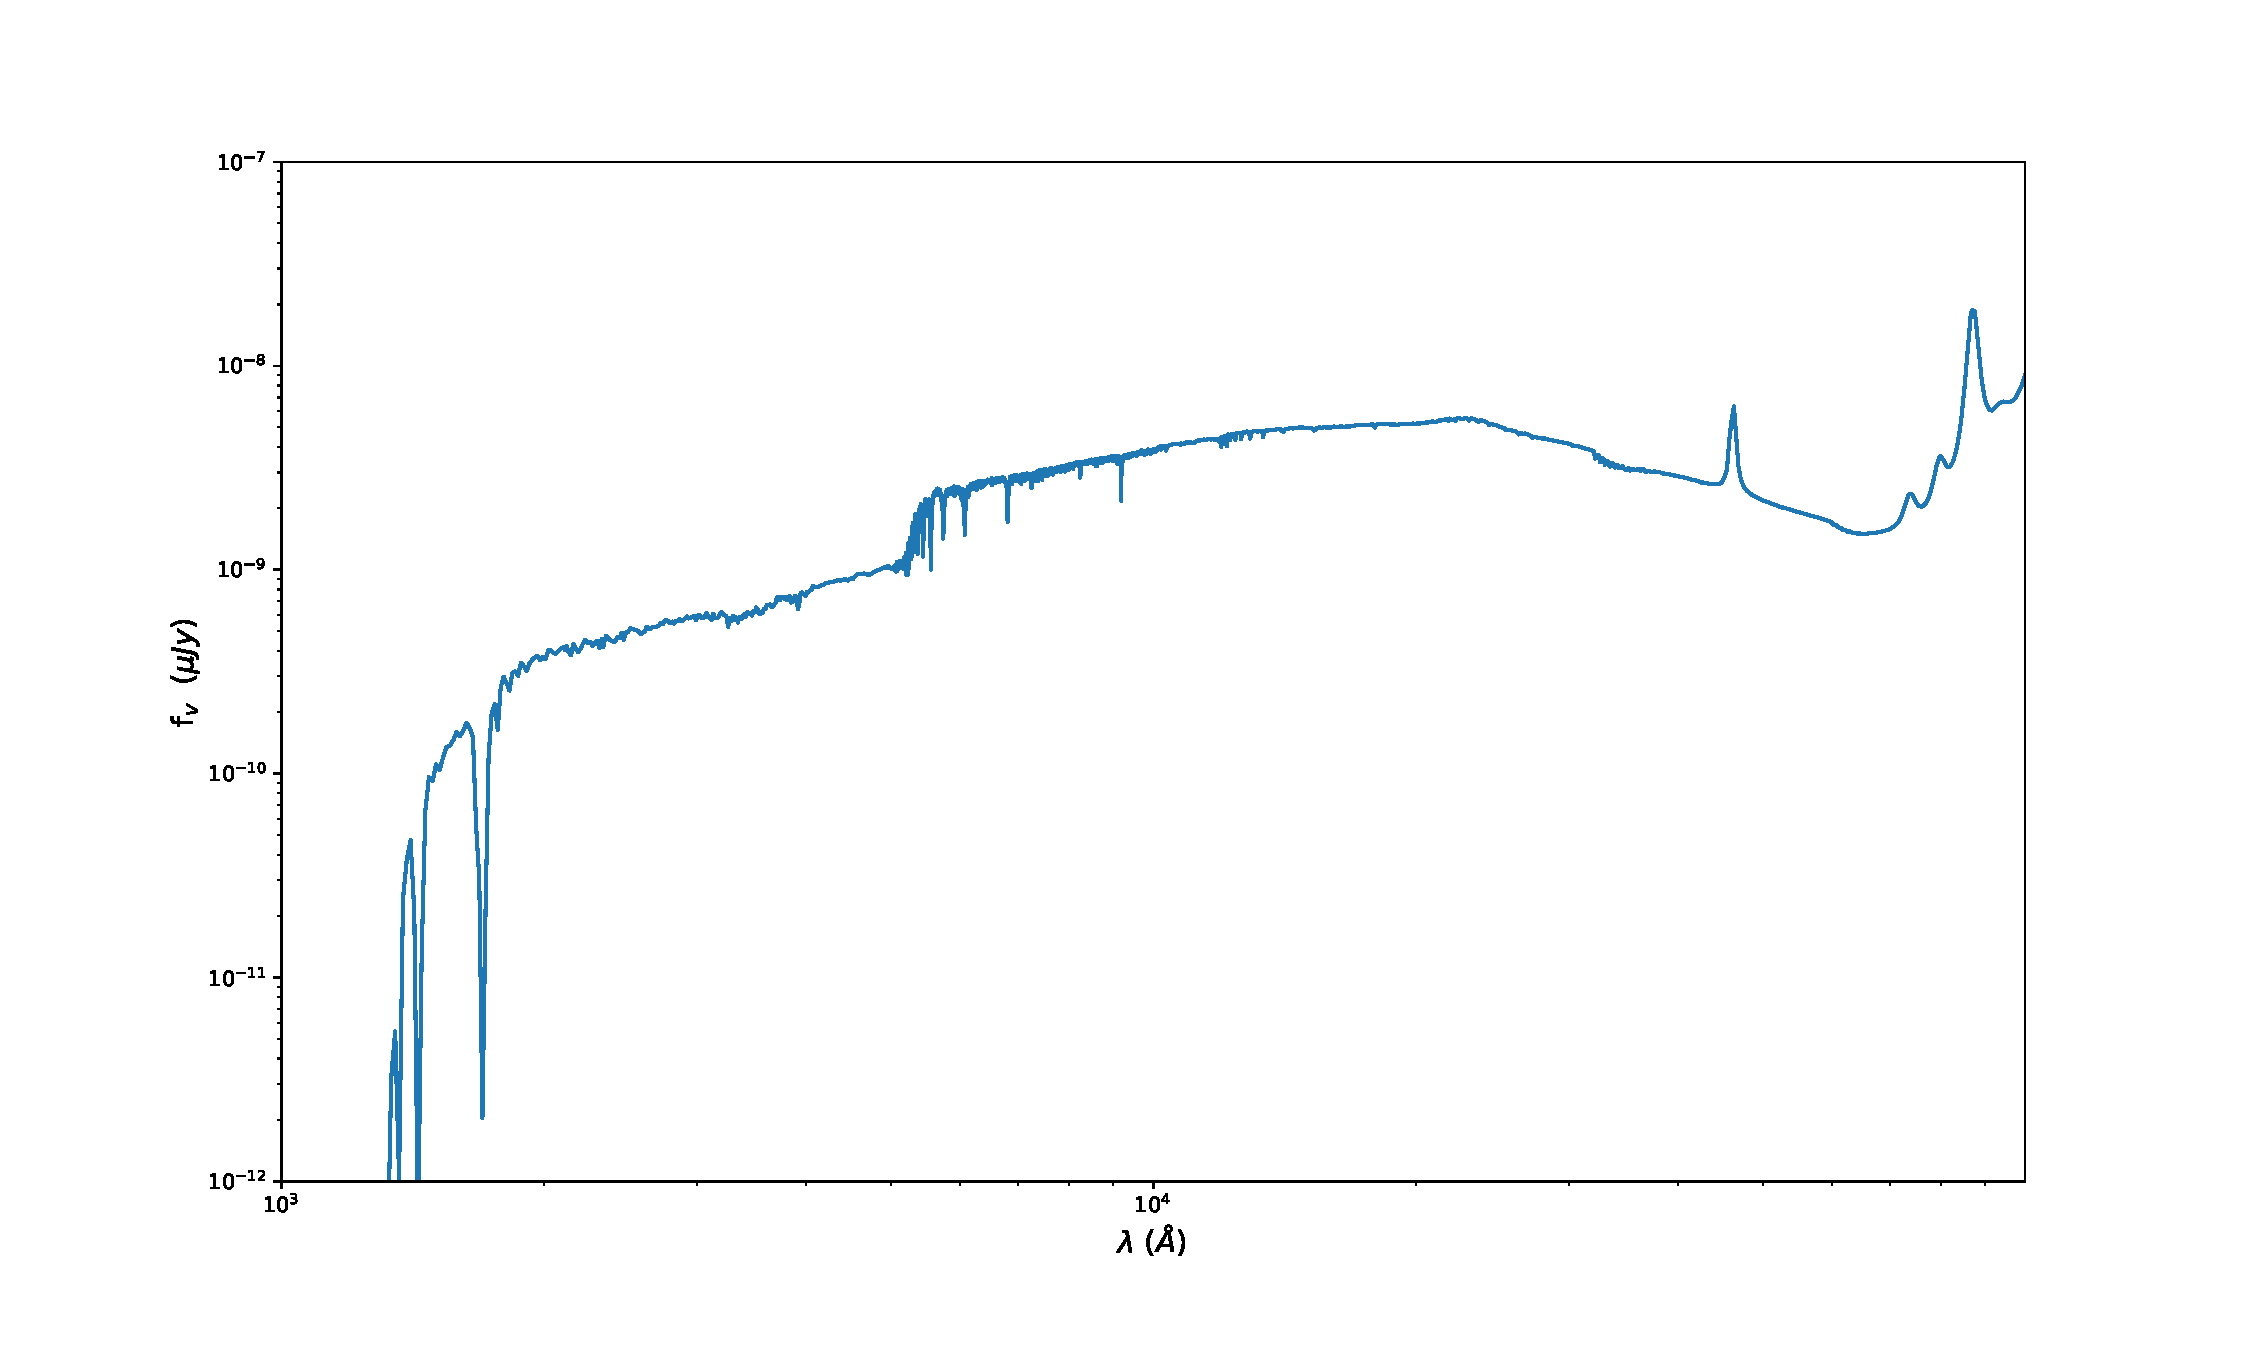
\includegraphics[scale=0.25]{SED closest galaxy 1}
\caption{SED of closest galaxy to galaxy 1 found by brute force}
\end{figure}

\begin{figure}[H]
  \centering
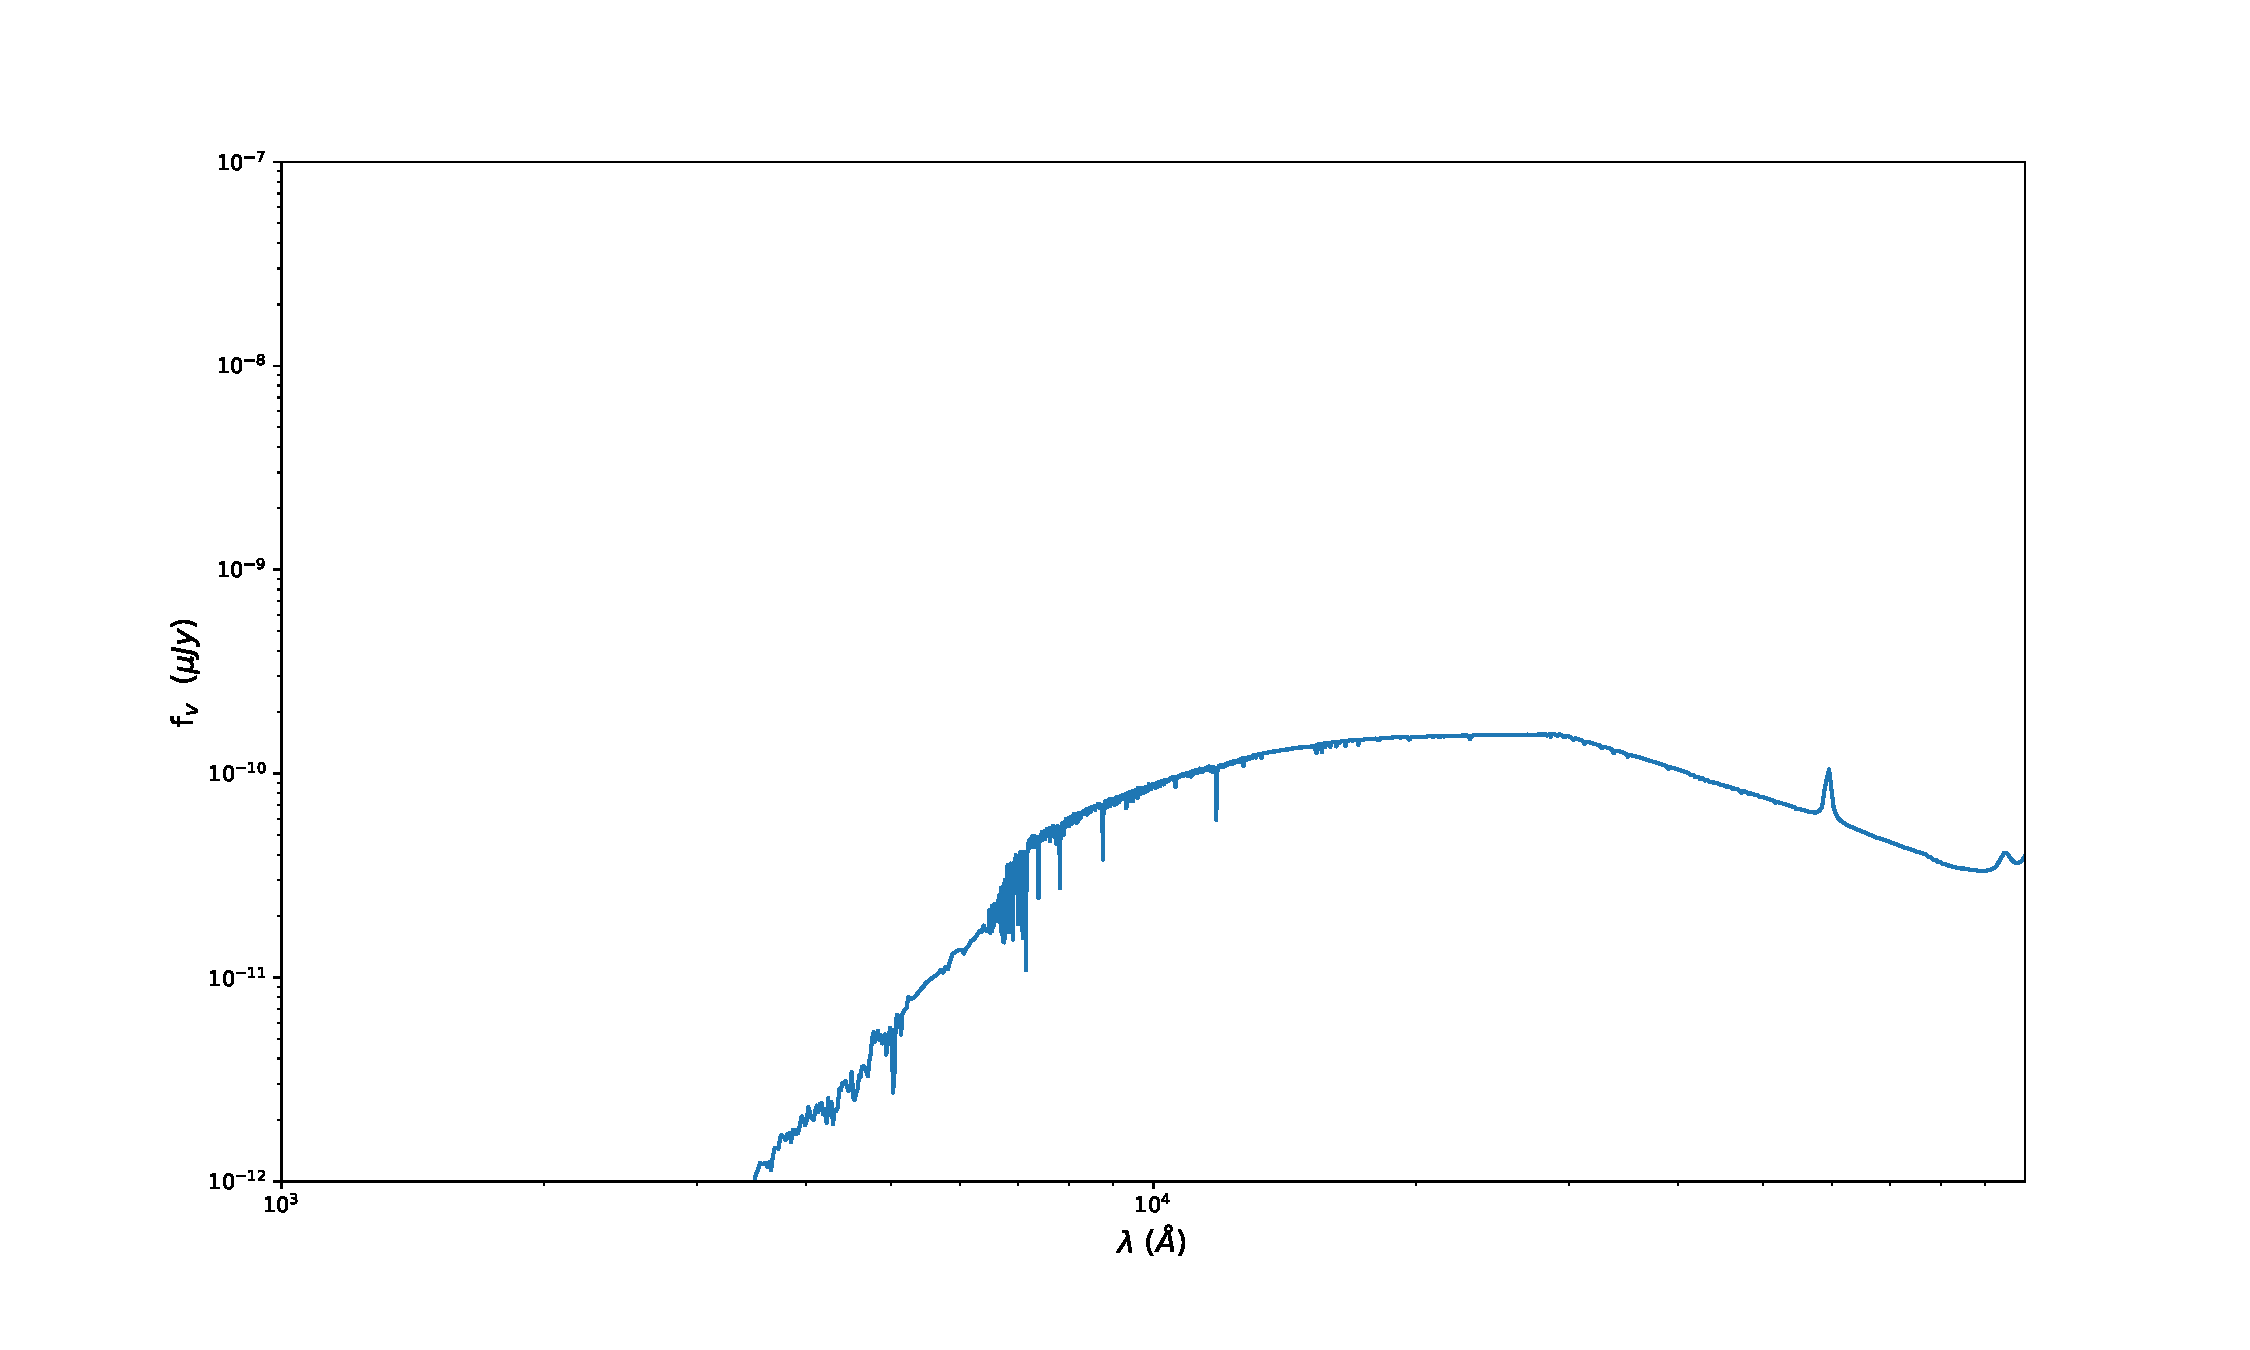
\includegraphics[scale=0.25]{SED closest galaxy 2}
\caption{SED of closest galaxy to galaxy 2 found by brute force}
\end{figure}

As you can see, the graphs are somewhat similar but have their discrepancies. Before continuing, one
should note that this is not a great way of approximating the age and redshifts of these galaxies.
In fact, we have no guarantees that we are even close to correct, we may have simply found a local
max of the likelihood function. To do this in a more intelligent way, Markov chain Monte Carlo
(MCMC) methods were used. First, MCMC was applied to the example of fitting a line. Of course,
applying MCMC to the the $\chi ^2$ model is pointless because we have an analytic solution. Instead,
we now adopt a more complex model with the assumption that the errors were somewhat underestimated.

\begin{figure}[H]
\[\ln({p}) = -\frac{1}{2} \sum_{i=1}^{N = 1} \frac{(y_i - f(x_i))^2}{s_i^2} + \ln({2\pi s_i^2})\]
\[ s_i^2 = \sigma_{i}^2 + f_0^2 f(x_i)\]
\caption{Likelihood function for new model}
\end{figure}

Notice that this model has a so-called nuisance parameter $f_0^2$. Because it is now not clear that
there is an analytical solution or even how f, m, and b (of course, $f(x_i) = m*x_i + b$) should
relate, MCMC is useful. To use MCMC, we define a uniform prior probability function, and use python
emcee's features. With 32 walkers centered around the values found from weighted linear least-square fitting and
10000 steps we get the following Markov chain.

\begin{figure}[H]
  \centering
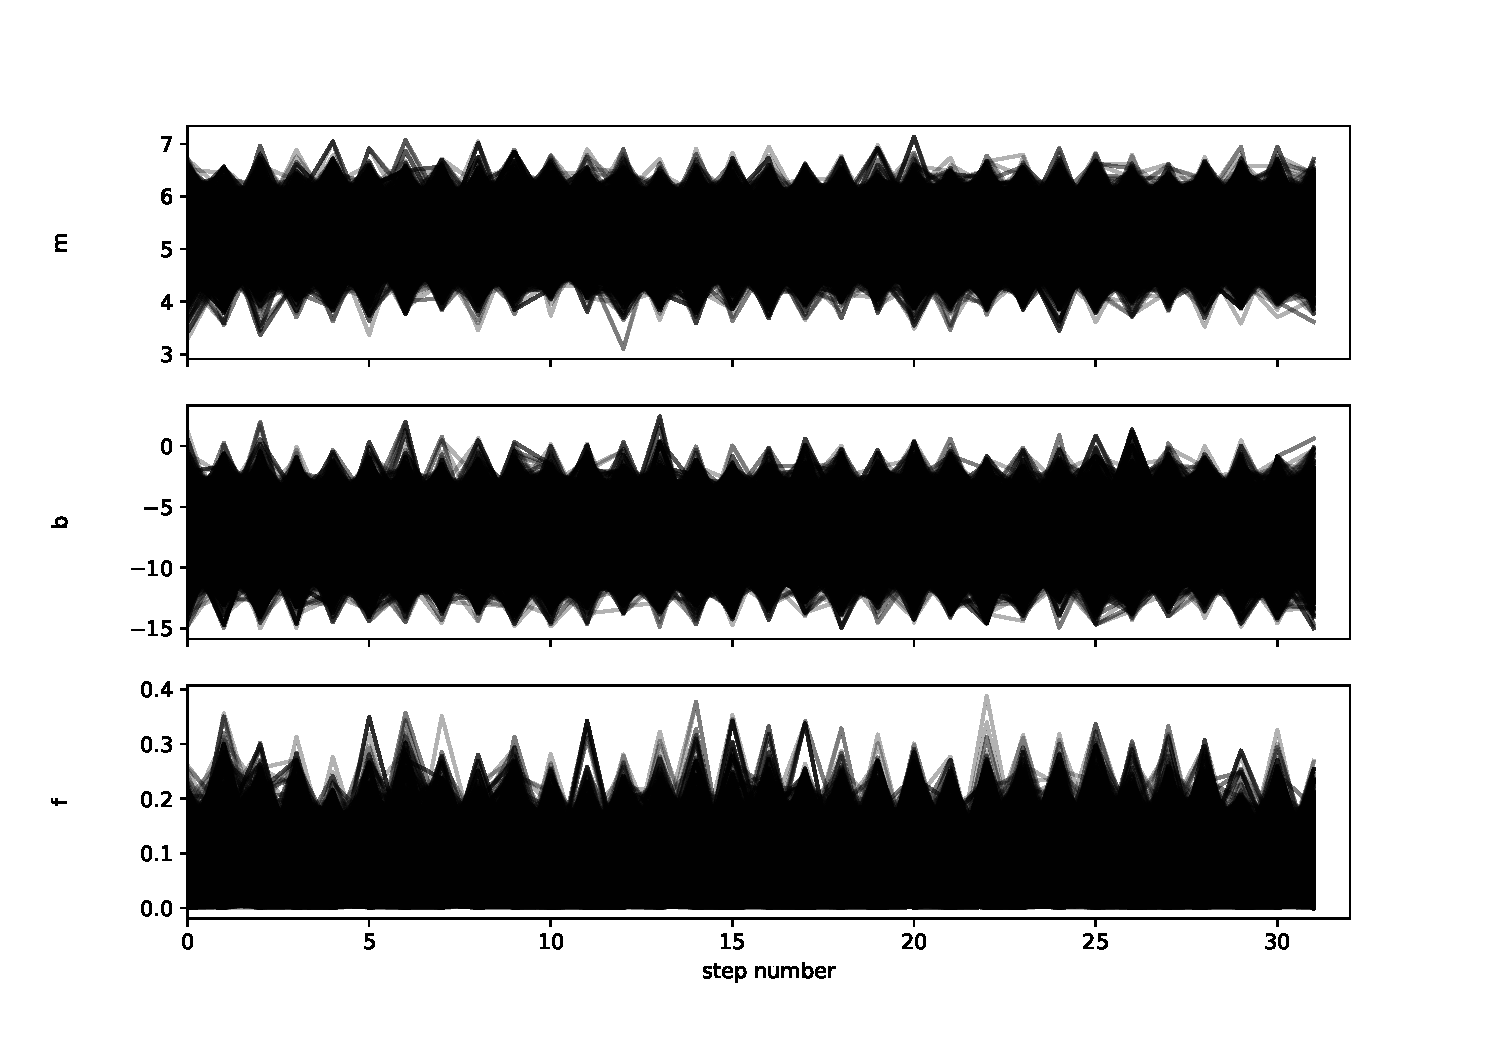
\includegraphics[scale=0.3]{Markov Chain}
\caption{Markov chain with emcee}
\end{figure}

According to the autocorrection time, it takes about 40 steps for the Markov chain to burn in.
Removing the first 40 steps, we get the following corner plots.

\begin{figure}[H]
  \centering
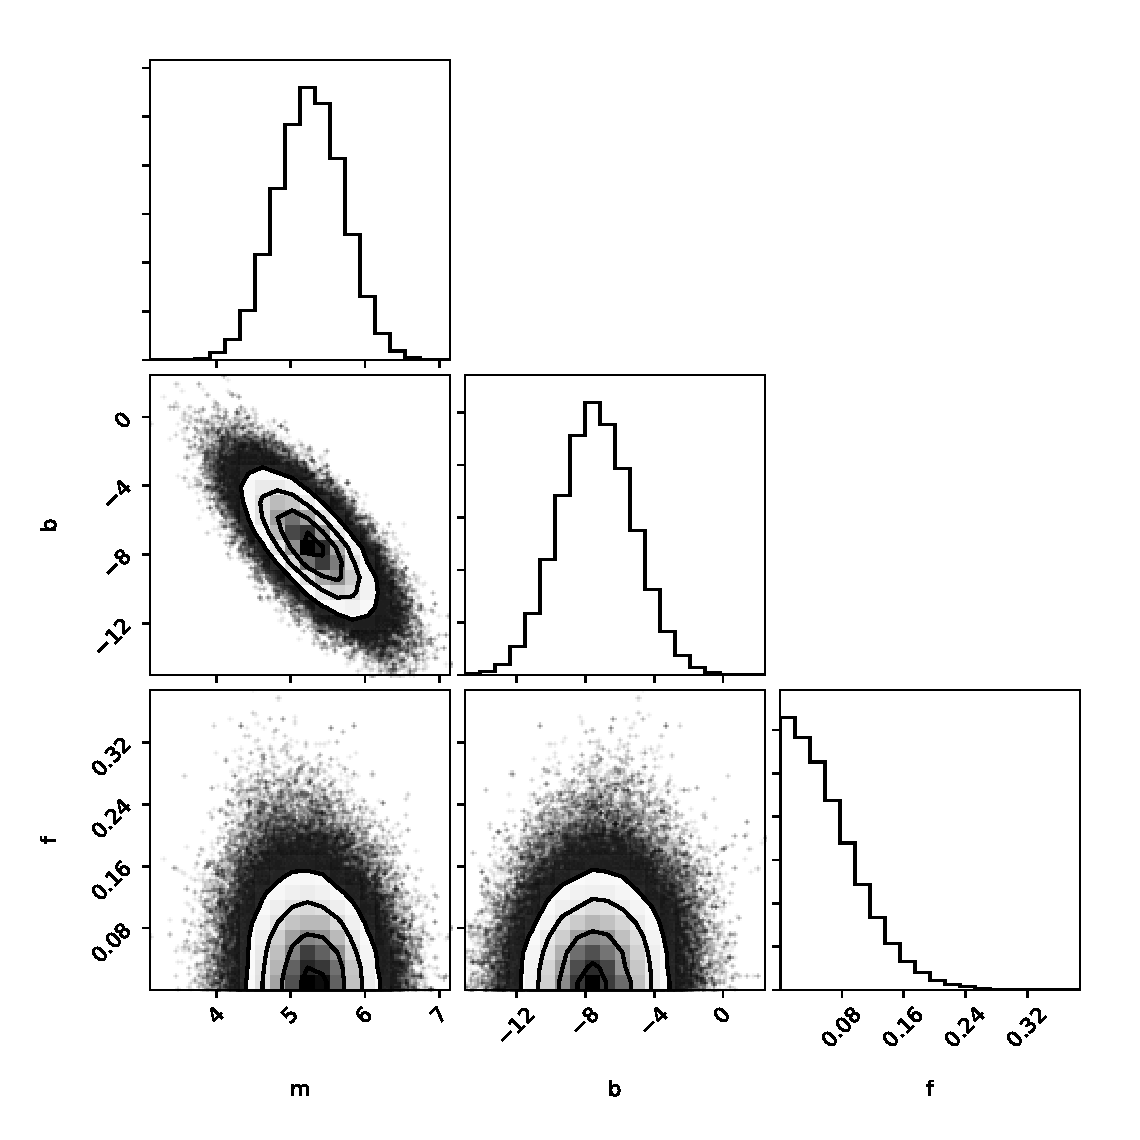
\includegraphics[scale=0.3]{Corner Graphs}
\caption{Markov chain with emcee}
\end{figure}

These plots show that b and m are closely related while b and f/m and f/b are not. The fact that f
takes on low values shows that the the errors are likely not underestimated by very much, if at all. Nonetheless, MCMC gives the following values for b, m, and f and graph.

$$m = 5.261^{+0.444}_{-0.455}$$

$$b = -7.391^{+2.172}_{-2.108}$$

$$f = 0.052^{+0.056}_{-0.037}$$

\begin{figure}[H]
  \centering
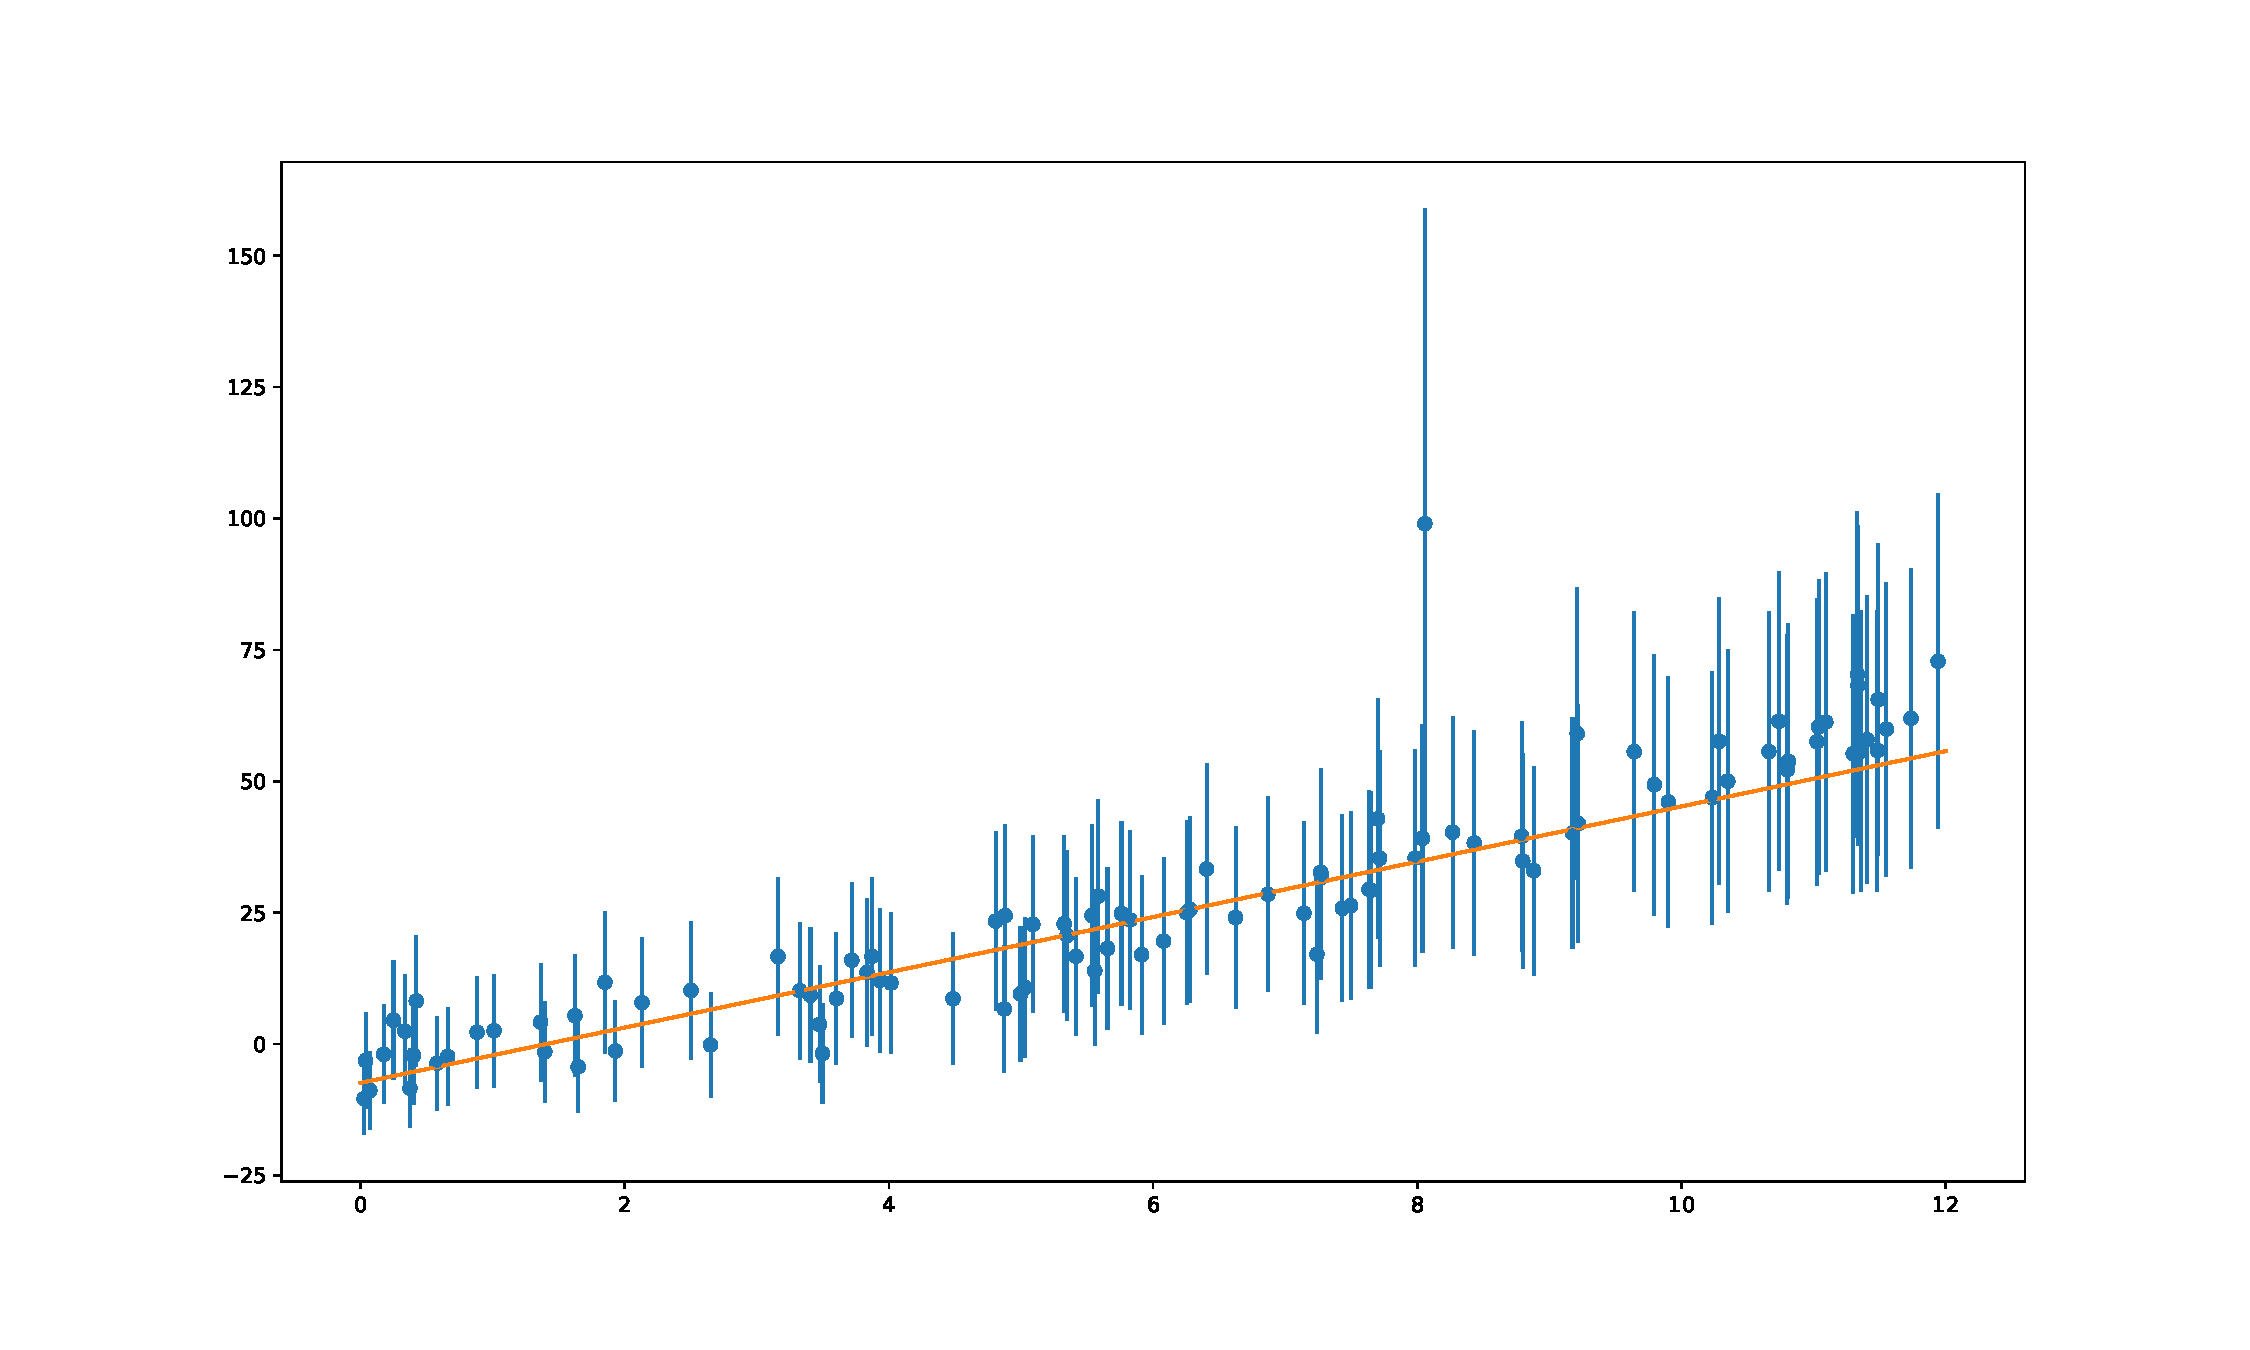
\includegraphics[scale=0.2]{Data and line 2}
\caption{Markov chain with emcee}
\end{figure}

The slope, y-int and uncertainties of this line are similar to the those from the weighted linear
least-square fitting line. A similar method was used to find optimal age and redshift for galaxy
1 and 2. Again, a uniform prior was used and the same likelihood function from above was used. When run with 2500 steps and 16 walkers centered around the estimated ages and redshifts,
the walkers did not move around the space - they got stuck around the estimated values. So, instead,
the walkers were started in random locations distributed around the estimated values. Here are the Markov
chains and corner plots.


\begin{figure}[H]
  \centering
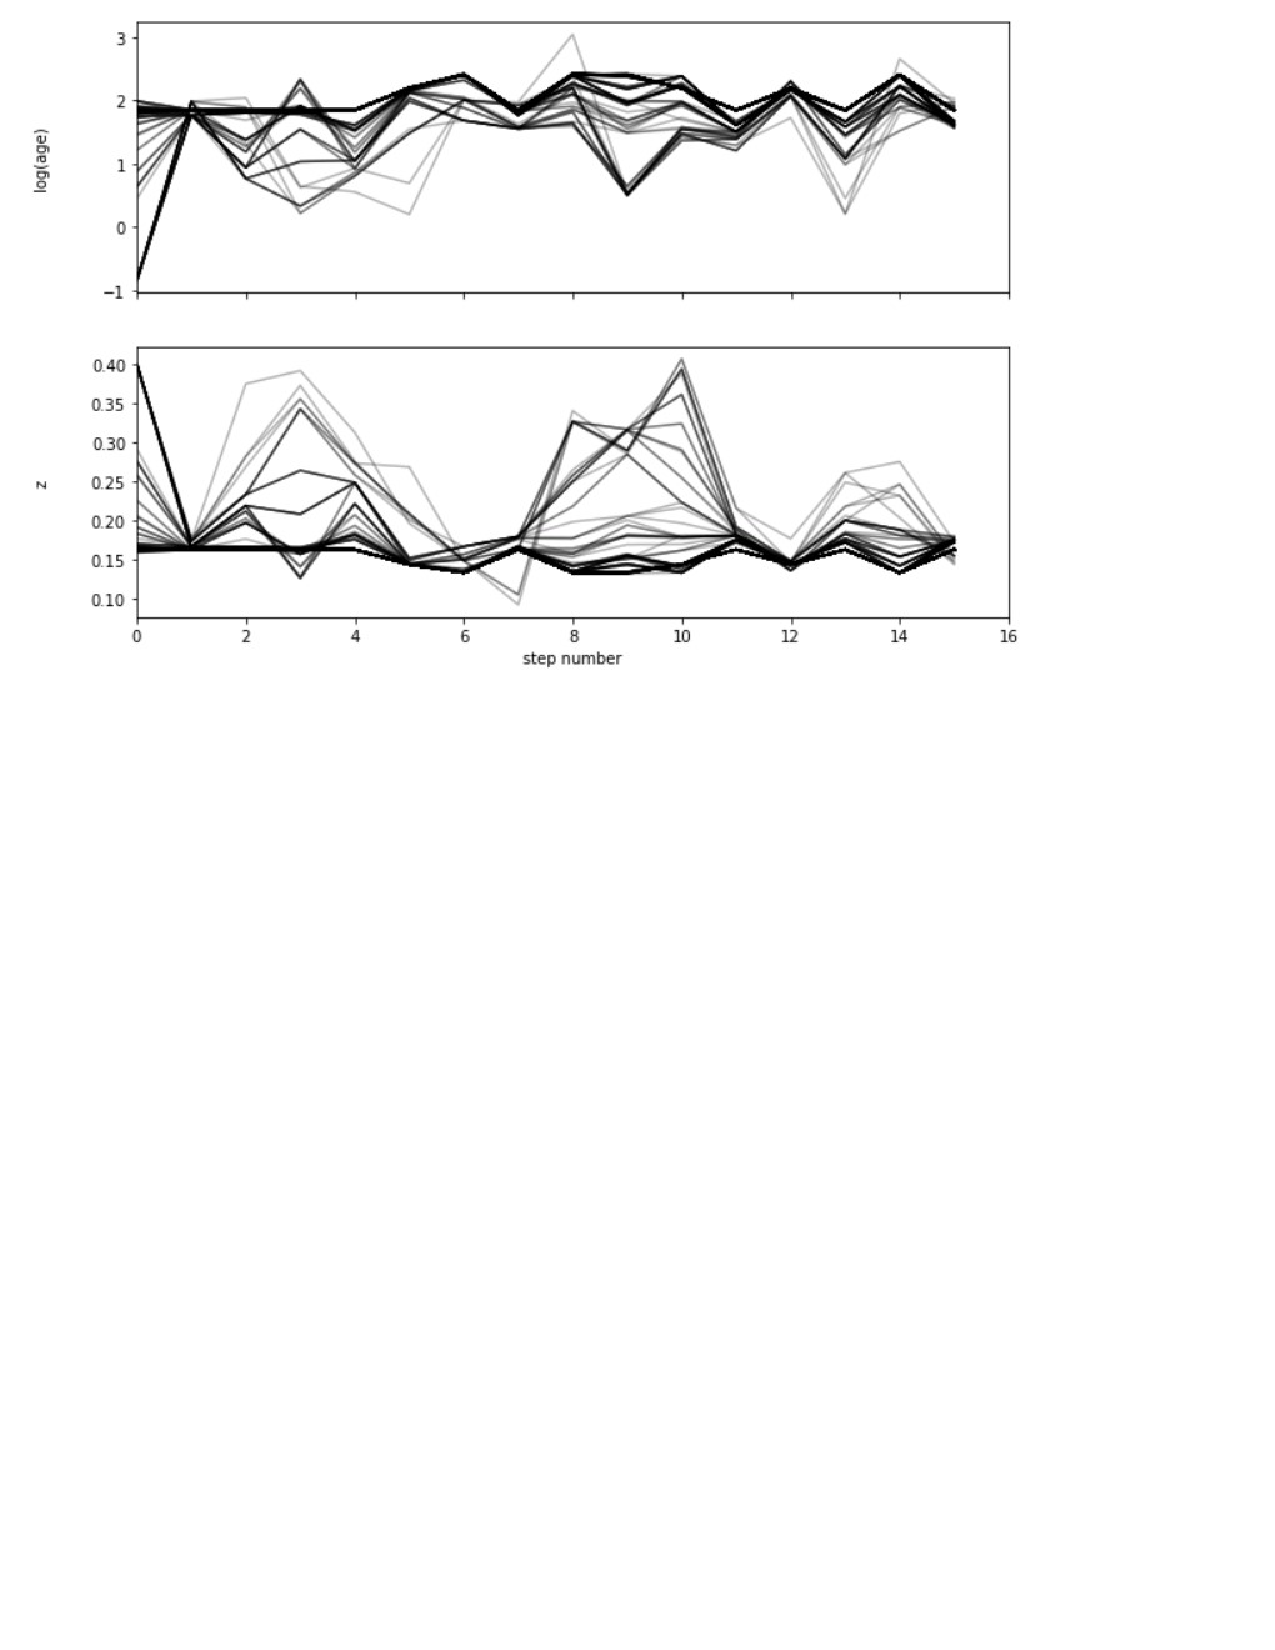
\includegraphics[scale=0.5]{Markov chain Galaxy 2}
\caption{Markov chain of galaxy 1 data with emcee}
\end{figure}

\begin{figure}[H]
  \centering
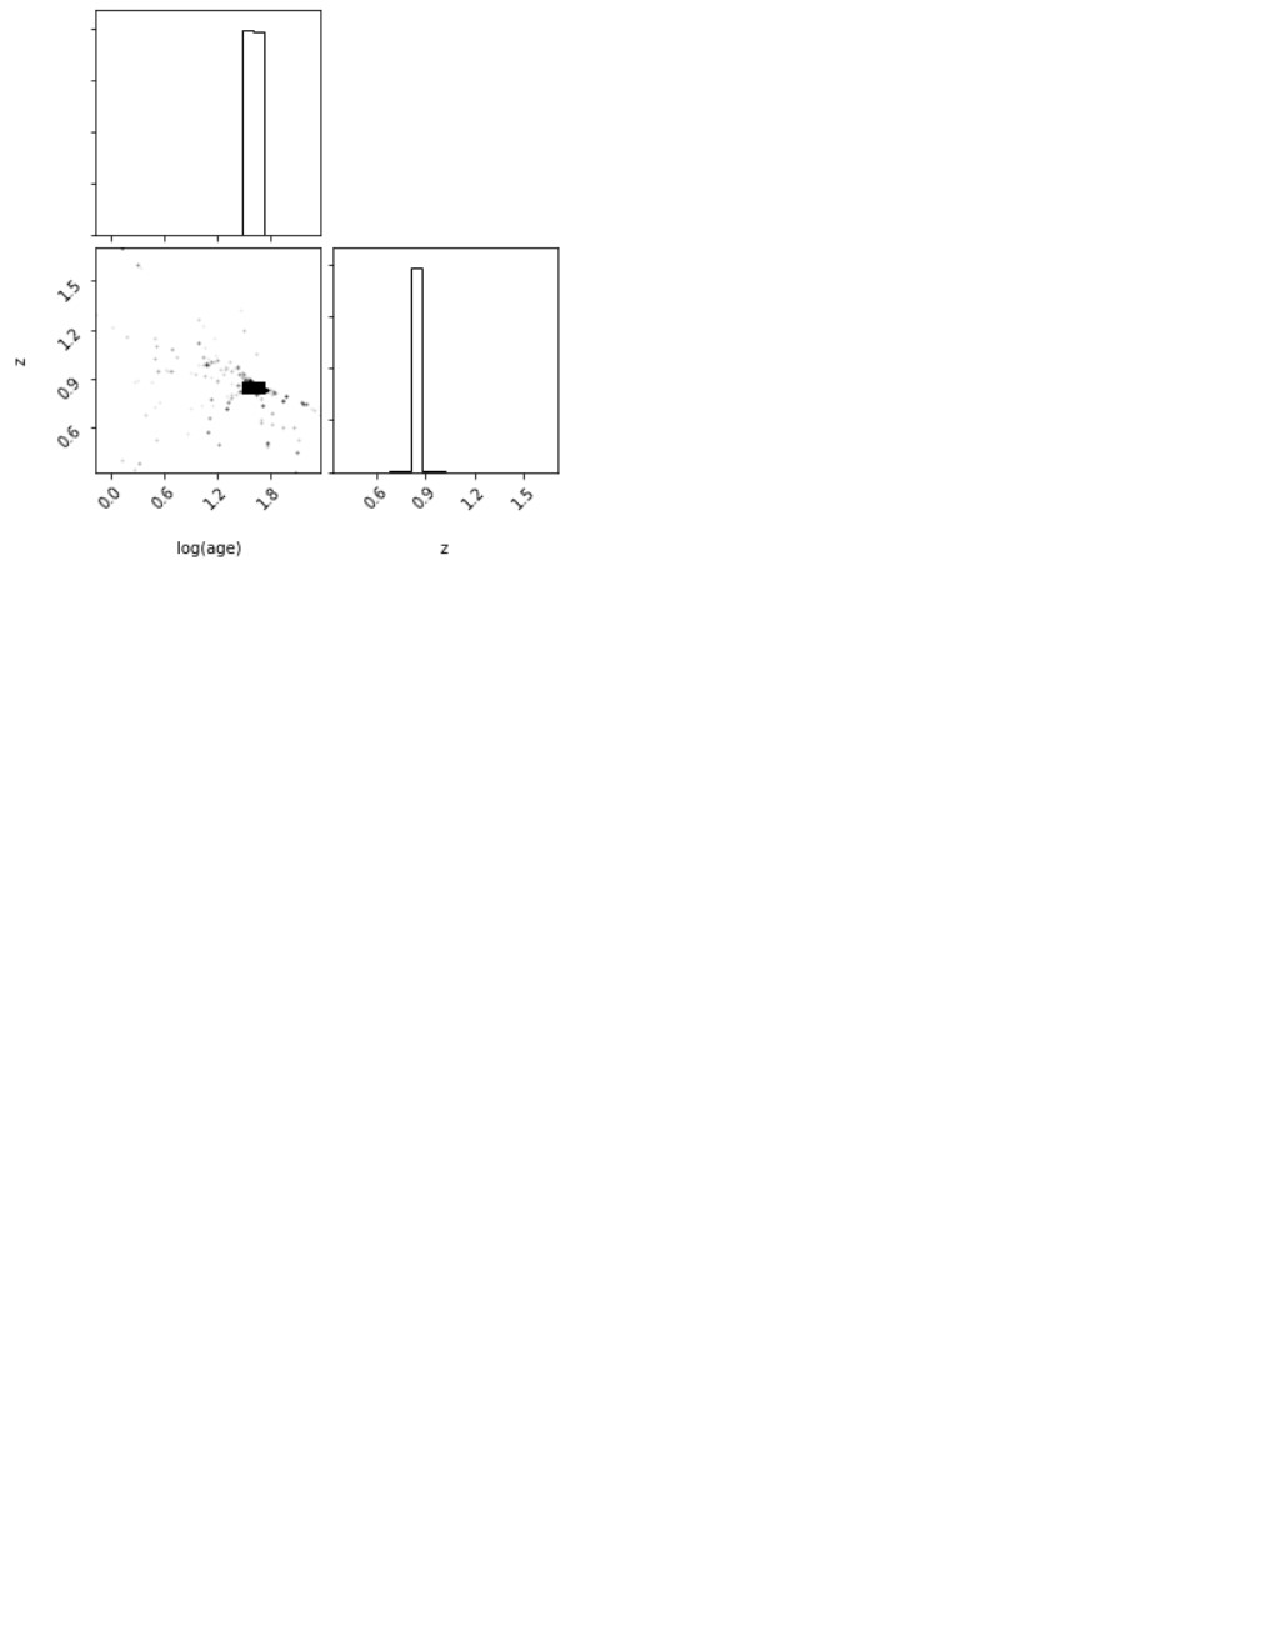
\includegraphics[scale=0.5]{Corner Graph Galaxy 1}
\caption{Corner graph of galaxy 1 data with emcee}
\end{figure}

$$ln{\textrm(age)} = 1.608^{+0.105}_{-0.002}$$

$$z = 0.853^{+0.016}_{-0.024}$$

Note that the error is likely somewhat higher than calculated here (which is due to how the distribution looks).

\begin{figure}[H]
  \centering
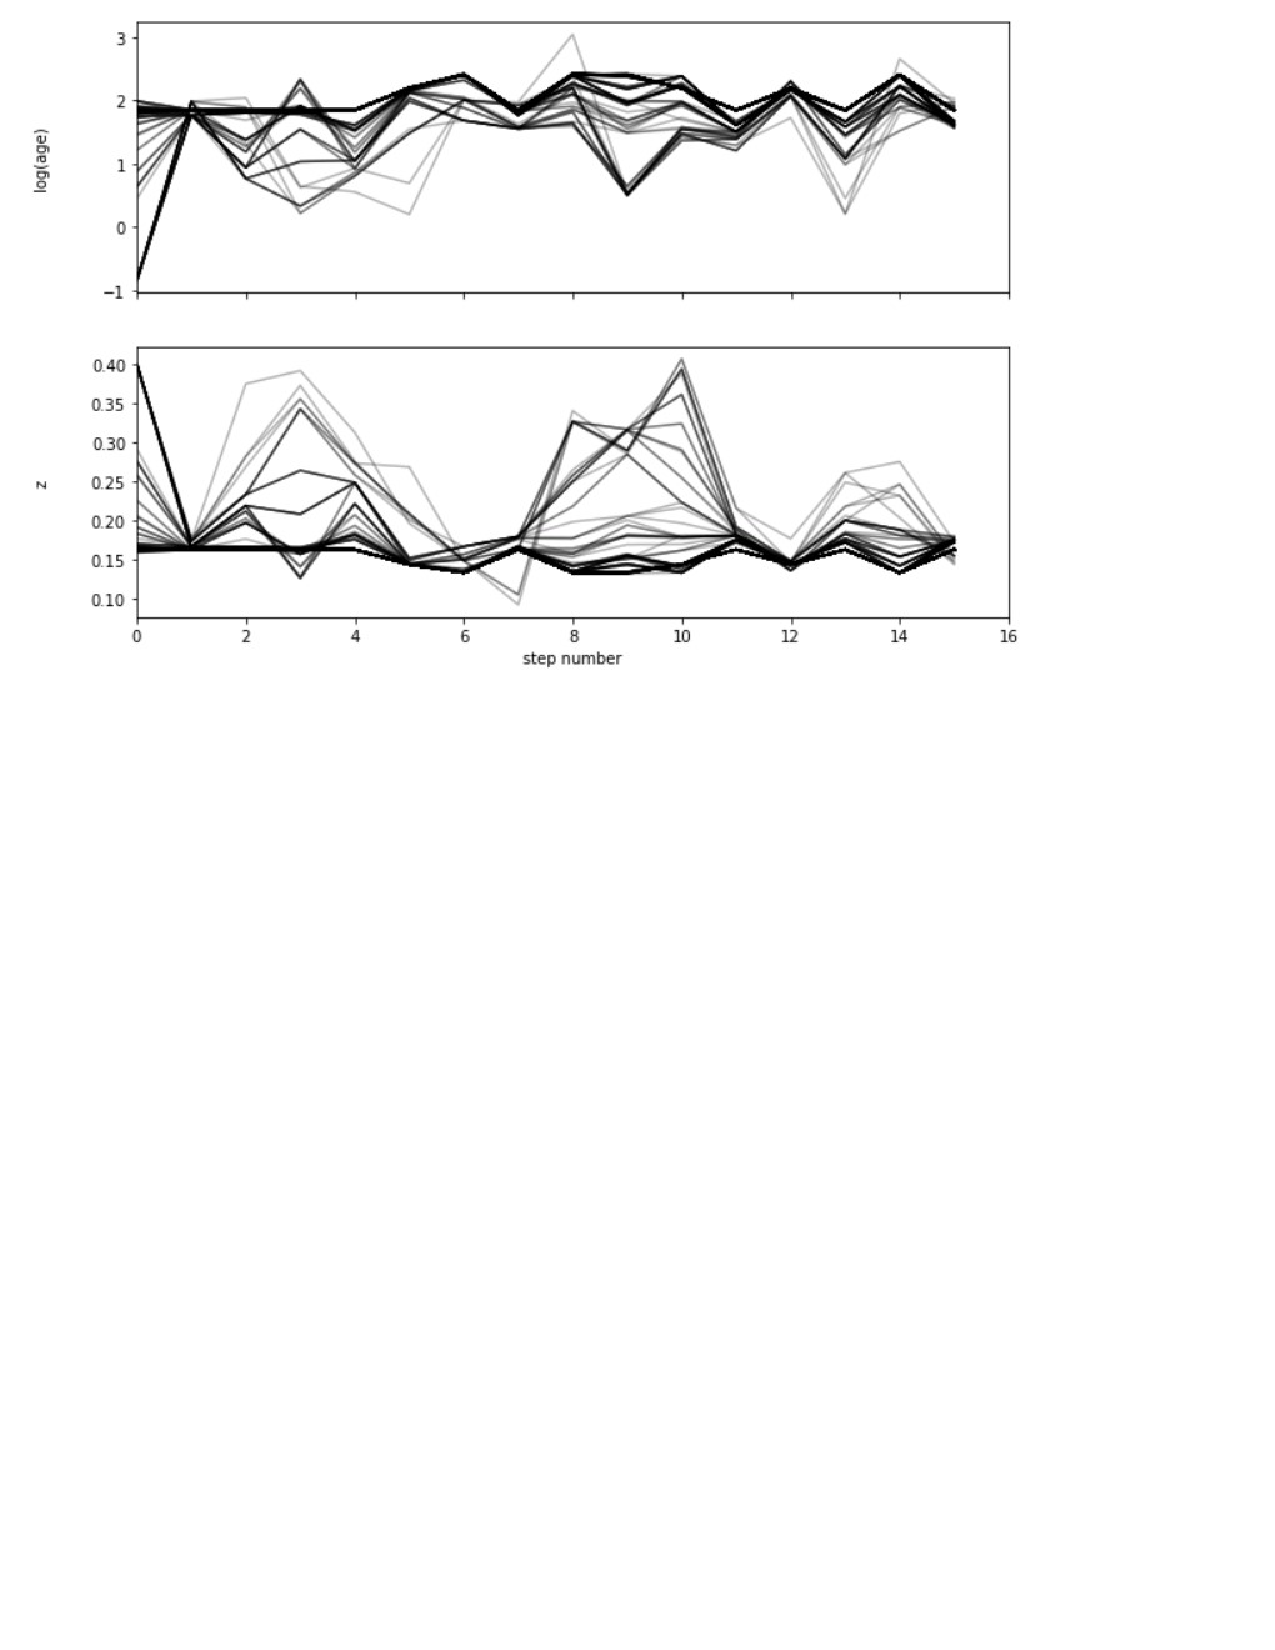
\includegraphics[scale=0.5]{Markov chain Galaxy 2}
\caption{Markov chain of galaxy 2 data with emcee}
\end{figure}

\begin{figure}[H]
  \centering
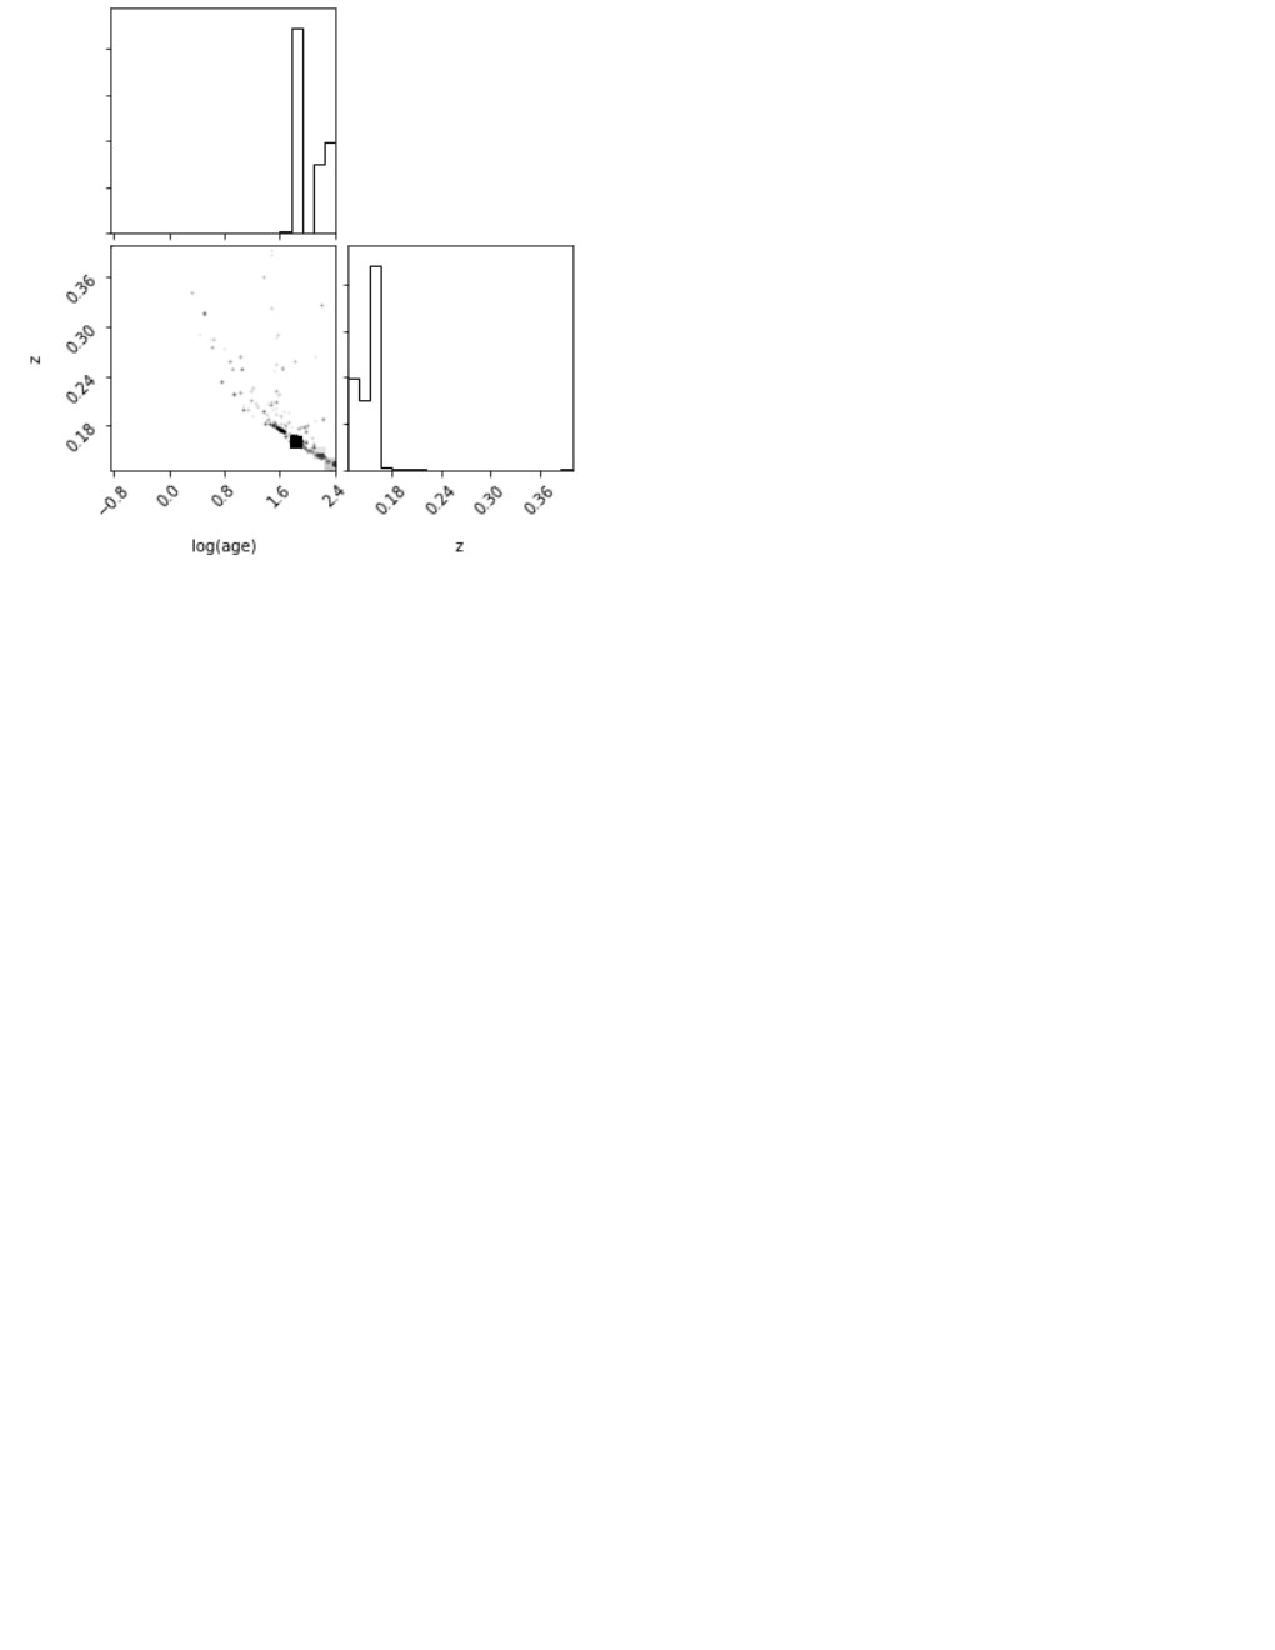
\includegraphics[scale=0.5]{Corner Graph Galaxy 2}
\caption{Corner graph of galaxy 2 data with emcee}
\end{figure}

$$ln{\textrm(age)} = 1.843^{+0.559}_{-0.001}$$

$$z = 0.162^{+0.000}_{-0.029}$$

Due to the difficulty of calculation, the Markov chain and corner plots were not as continuous but it is
interesting how they still find a similar answer to the brute force method

The next step would be to add stellar mass and dust attenuation to the free variables in MCMC.
Though it would be easy to extend the code to do this, the MCMC calculations above already
took several hours, so, this would undoubtedly take unreasonably long in the current setup. To make
this feasable, one could use the Scinet cluster or try to further optimize the code.

\subsection*{Question Answers}

\paragraph{1.0.} As briefly mentioned in the introduction, stellar population synethsis (SPS) refers to
combining information on stellar evolution, calibrated stellar libraries, initial mass functions
(IMF), and dust in the interstellar medium to construct the SED of a galaxy. Many different SPS models exist,
and they  have their own assumptions, tools, and calibrations. By using an SPS model, specifying a
galaxy's physical properties allows for reconstructiion of its SED. Of course, this is only half the battle
because we would like to go from the SED to a galaxy's physical properties. There have been many approaches to
solving this problem, including Monte Carlo methods, machine learning, and numerical methods. No matter
the tool used, the role of the SPS model is the same. The SPS model will generate SEDs given specified physical
parameters which will be compared to the SED of the desired galaxy (there are many ways to "compare," of course).
Then, adjustments will be made to the physical parameters in hopes of finding a better fit between the generated
and desired SED. In this way, SPS models provide the foundation for this method of determining a galaxy's
physical properties from its emitted light.

\paragraph{1.3.} The StellarPopulation can take in a variety of inputs about the galaxy, including its dust
content, initial mass function, metallicity, the type of star formation history and more.

\paragraph{1.4.} As discussed above, the units of the output spectrum are solar luminosity per hertz
($L_\odot/Hz$). The StellarPopulation object is using MESA Isochrones and Stellar Tracks (MIST) and
the MILES spectral library. At 100 Myr, the stellar mass of the galaxy is about 0.92 $M_\odot$.

\paragraph{1.7.} As galaxies cannot be older than the universe, when a galaxy is observed at some redshift
$z$, we are effectively looking back in time $t$ at its light. Then, $t + t_g < t_u$ (there are equations
to calculate $t$ from $z$) where $t_u$ is about 13.8 billion years. So, the larger a galaxy's redshift,
the smaller its possible maximum age is.

\paragraph{2.1} There are many possible techniques to fit a straight line to a set of sampled
points. As Hogg, Lang, and Bovy point out, the standard method when there is negligible error in the x
data and known Gaussian error in the y data is weighted linear least-square fitting. This type of fitting minimizes $\chi ^2$ which can be intuitively understood as a measure of
the line from the data. It is mathematically defined as:

$$\chi ^2 = \sum_{i=1}^{N = 1} \frac{(y_i - f(x_i))^2}{\sigma_{yi}^2}$$

Part of the motivation for using this measure of goodness of fit is that it has an easily calculable
minimum with linear algebra. With this method, we get a reasonable looking line of best fit. It is
difficult to say whether a line is the best curve to represent the data without any physical
knowledge about the data, however, a line appears to fit the data well with a relatively low $\chi
^2$.

\end{document}
